% !TeX root = ../main.tex

\chapter{HALF设备保护系统的设计}

\section{HALF预研工程}

HALF是一个位于中低能区,以真空紫外和软X射线为主的,具有高亮度、低发射度和全辐射谱段空间相干性最先进的衍射极限光源。HALF将集成与相干性密切关联的系列先进测量技术,具有超快时间分辨、超高空间分辨和超高能量分辨的能力,为量子信息与量子材料、能源与环境、物质科学、生命科学等前沿研究领域提供强有力的研究平台。

目前国家同步辐射实验室在中国科学院和地方政府的共同支持下开展了HALF预研工程,预研工程将对加速器、光束线站的核心关键技术进行攻关及样机研制,为未来HALF的建设打好技术基础。HALF预研工程计划于2020年底完成,目前最新设计的HALF结构如图~\ref{fig:half-arch}所示,HALF加速器总体由注入器和储存环组成。

\begin{figure}[!htb]
	\centering
	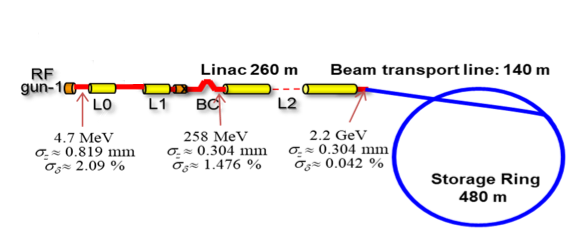
\includegraphics[width=0.9\textwidth]{half-arch.png}
	\caption{HALF总体结构图}
	\label{fig:half-arch}
\end{figure}

注入器由满能量直线加速器(Linac)和束流输运线(Beam transport line)组成,其中直线加速器的长度为260米,输运线长度为140米。直线加速器用于产生电子束,将其能量加速器到2.2GeV。,输运线负责将直线加速器的电子束传输到储存环,沿储存环切线方向产生的同步辐射光通过光束线传输到实验站进行各种科学实验。

HALF储存环的光束发射度非常小,因此光束线可以将一定波长范围内的光束聚焦到其衍射极限,这种类型的储存环称为衍射极限储存环,HALF衍射极限储存环的最新设计参数如表~\ref{table:4.1}所示。

\begin{table}[!htb]
	\centering\small
	\caption{HALF储存环主要参数值}
	\label{table:4.1}
	  \begin{tabular}{ccc}
		  \toprule
		  参数        & 数值 & 单位\\
		  \midrule
		  能量  &  2.2  & GeV \\
		  周长  & 480  &  m \\
		  周期数  & 20 & - \\
		  自然发射度  & 85.1  &  pm $\cdot$ rad \\
		  工作点(H/V)  & 48.175/17.175  & - \\
		  自然色品  & -75, -79  &  - \\
		  动量紧缩因子   & $6.3\times 10^{-5}$  &  - \\
		  阻尼分配数(H/V/L)  &  1.475/1.0/1.525  & -  \\
		  自然阻尼时间(H/V/L)  & 22/32.4/21.2  & ms \\
		  电子单圈弯铁辐射能量损失 & 217.5  &  keV \\
		  自然能散  & $0.66\times 10^{-3}$   & - \\
		  直线节数目  & 40个(20个长直线节+20个中直线节)& - \\
		  长直线节长度  & 5.5& m \\
		  长直线节中点处的$\beta_{x}$/$\beta_{y}$/色散函数 & 5.445/2.533/0.0 & m \\
		  中直线节长度  & 2.2 & m \\
		  中直线节中点处的$\beta_{x}$/$\beta_{y}$/色散函数  & 2.842/1.954/0.028 & m \\
		  \bottomrule
	  \end{tabular}
\end{table}

\section{加速器中的设备保护系统}

\subsection{设备保护系统的任务}
机器保护系统(Machine Protection System,MPS)是加速器控制系统的重要组成部分,负责保护加速器机器组件的安全。MPS在加速器各分总体、系统之间建立联锁保护逻辑,当设备出现故障或者束流丢失时,MPS能够快速地对加速器重要设备实施保护,并向中央控制系统报告设备故障信息,对故障数据进行存档和分析。根据响应时间的不同,MPS可分为慢联锁保护系统(Slow Protection System,SPS)和快联锁保护系统(Fast Protection System,FPS),SPS和FPS在不同加速器装置中的名称有所不同,例如ALBA光源将SPS称为设备保护系统(Equipment Protection System,EPS),将FPS称为FIS(Fast Interlock System)\cite{Alba-eps}。本文将HALF MPS中的慢联锁保护系统称为EPS,快联锁保护系统称为FPS。从系统响应时间的角度来看,EPS的响应时间一般在10ms量级,而FPS的响应时间一般要求在10$\mu$s量级。EPS和FPS的具体应用场合如下:

(1) EPS监测的设备状态信号主要是真空度、温度、冷却水流量等与设备运行安全相关的信号,经过EPS联锁逻辑判断后,迅速实施相应的设备保护措施。

(2) FPS的应用场合是在加速器运行过程中,如果发生了束流偏离轨道达到一定阈值或者某些设备出现故障,导致电子束流可能会损毁机器,此时必须采取保护措施及时切断束流。

\subsection{国内外加速器的机器保护系统调研}
本节对国外加速器装置机器保护系统的结构和硬件组成进行了调研,具体情况如下:

\subsubsection{LCLS的机器保护系统}

直线加速器相干光源(Linac Coherent Light Source,LCLS)是世界上第一个硬X射线自由电子激光装置,其永磁波荡器长度为130米,位于美国斯坦福直线加速器中心。LCLS机器保护系统的任务是避免波荡器等重要设备受到束流照射而损坏,要求MPS在一个束流脉冲周期8.33ms内切断束流。MPS监测的信号包括束流损失信号、束流位置信号、束流强度和插入件状态。

LCLS机器保护系统的系统架构如图~\ref{fig:lcls-eps-arch}所示,机器保护系统由32个从节点(Link Node)和一个主节点(Link Processor)组成,主节点通过核心交换机与从节点构成星形拓扑结构,节点间通过专用的千兆以太网通信,通信协议是LCLS自主设计的实时协议。从节点分布于从激光注入器到X射线实验线站的整个装置,负责接收束流故障信号。主节点按照联锁保护逻辑处理来自从节点的束流故障信号,通过相应的控制设备(Mitigation device)切断束流。主节点和从节点同时接入到EPICS控制网络,用于中控系统监控机器保护系统的状态\cite{Norum-2009}。

\begin{figure}[!htb]
	\centering
	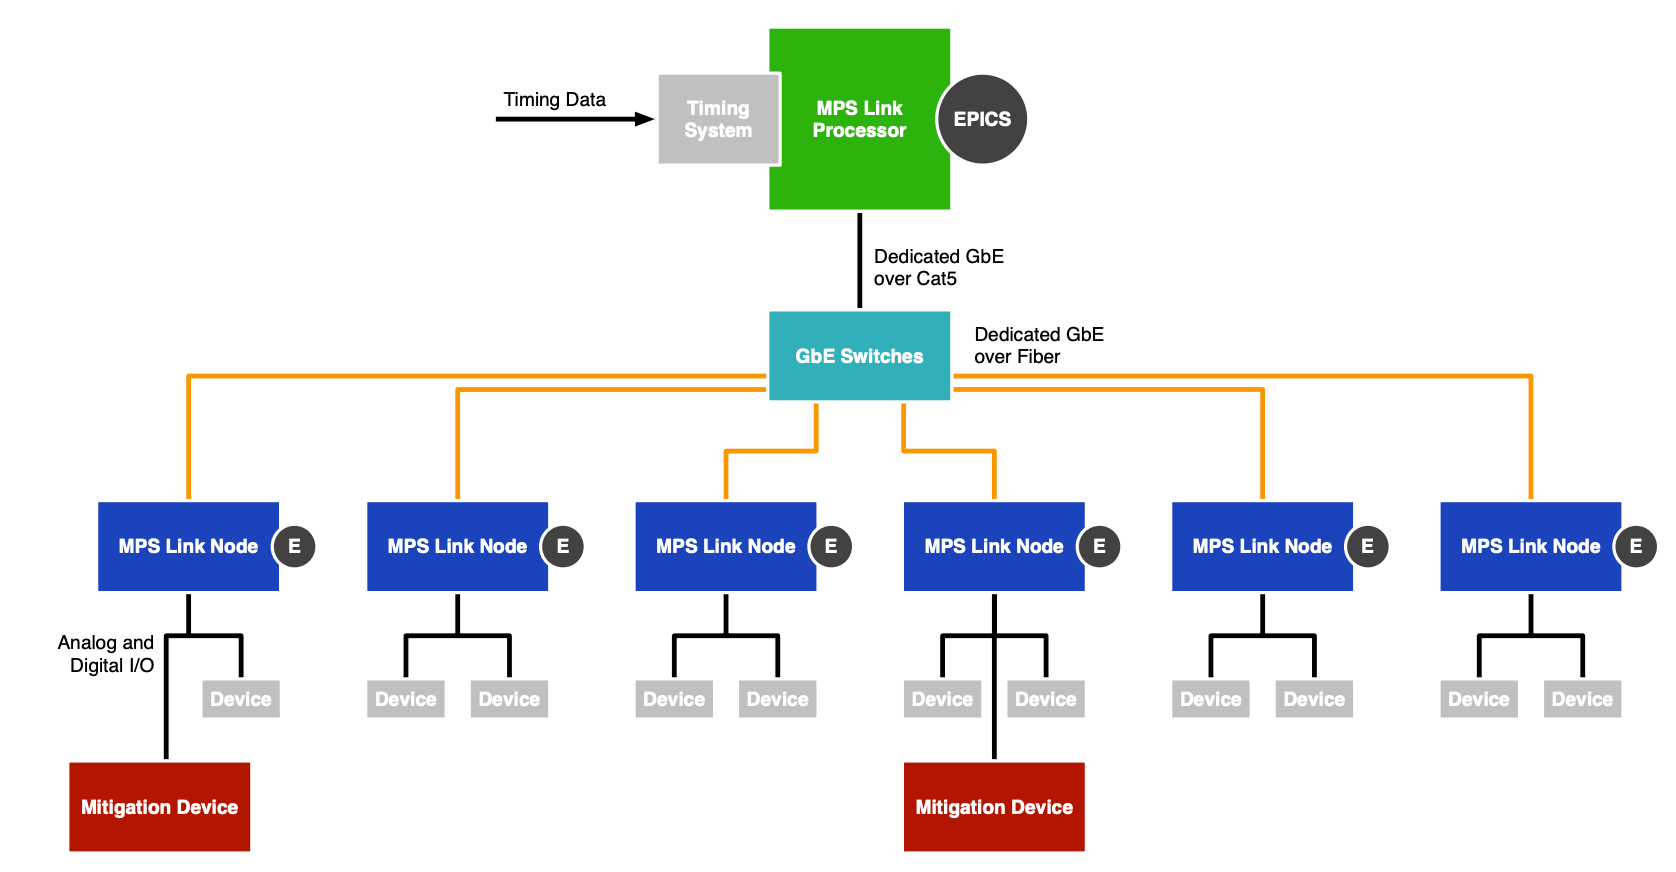
\includegraphics[width=\textwidth]{lcls-eps-arch.png}
	\caption{LCLS机器保护系统结构图}
	\label{fig:lcls-eps-arch}
\end{figure}

机器保护系统的从节点基于型号为Xilinx Vertex4的FPGA芯片实现,每个连接节点可支持多达96路数字输入,8路固态继电器输出,4路TTL兼容逻辑电平触发输入和4路触发输出,同时配备了单独的串口与EPICS IOC通信。

\subsubsection{RAON的机器联锁保护系统}

Rare isotope Accelerator complex for ON-line experiment(RAON)是一台正在建设中的重离子加速器,为在线同位素分离实验和飞行时间型碎片分离实验提供平台。RAON由韩国基础科学研究所(IBS)负责,CERN,Fermilab,TRIUMF等实验室也共同参与到RAON项目建设中。

RAON机器保护系统的结构如图~\ref{fig:RAON-eps-arch}所示,由Slow Interlock System(SIS)、Fast Protection System(FPS)、Beam Permit System(BPS)和Post-mortem System(PMS)组成\cite{hyunchang-2018},

\begin{figure}[!htb]
	\centering
	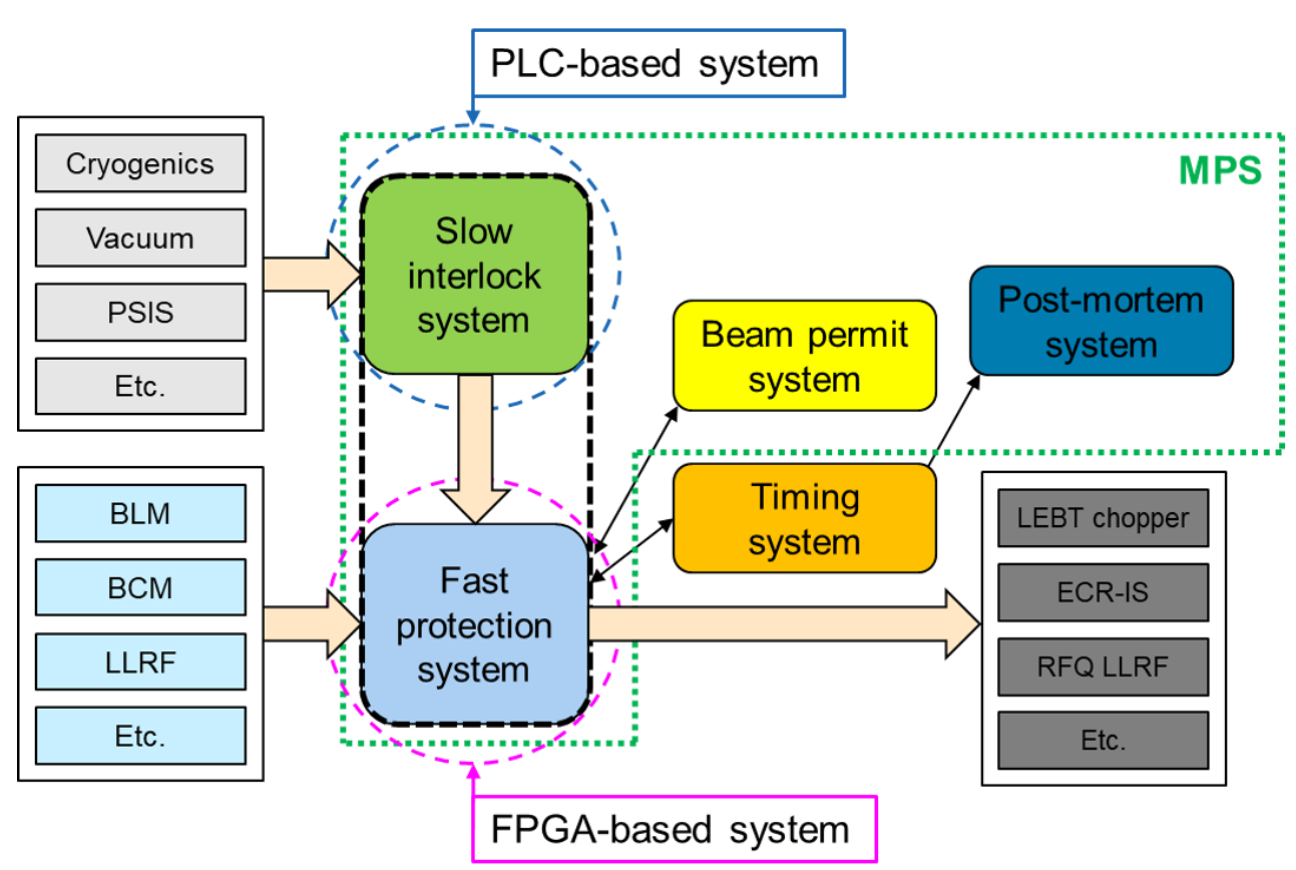
\includegraphics[width=\textwidth]{RAON-eps-arch.png}
	\caption{RAON机器保护系统结构图}
	\label{fig:RAON-eps-arch}
\end{figure}


各系统具体设计如下:

(1) SIS基于PLC实现,监测低温,真空等系统中的设备信号,一旦设备出现故障,SIS要在几十ms内通过FPS实施切断束流的设备保护措施。

(2) FPS各节点基于FPGA实现,FPS节点监测的信号来自束流丢失监测器(BLM)、束流流强监控器(BCM)、低电平(LLRF)系统设备等,FPS需要在几十$\mu$s内通过禁止高频功率输出等措施切断束流。

(4) BPS负责根据加速器不同的运行模式来切换MPS运行状态。

(5) PMS是用来对设备故障信号进行存档和分析的系统。

\subsubsection{上海光源储存环的机器保护系统}

文献\cite{yu2020}中所描述的机器保护系统是指上海光源的设备保护系统,基于PLC实现,其总体结构如图~\ref{fig:ssrf-eps-arch-1}所示,具体设计如下:原有的上海光源储存环机器保护系统由1个储存环分总体机器保护系统控制器和20个机器保护系统单元控制器组成,控制器采用日本Yokogawa FA-M3系列PLC,机器保护系统单元负责监控本单元的真空相关信号和冷却水状态信号,机器保护系统单元之间通过电缆相连。20个机器保护系统单元将各单元的联锁信号传输给储存环分总体级联锁控制器,经过储存环分总体联锁控制器逻辑判断后,给出禁止高频功率输出、禁止储存环注入等保护信号。

\begin{figure}[!htb]
	\centering
	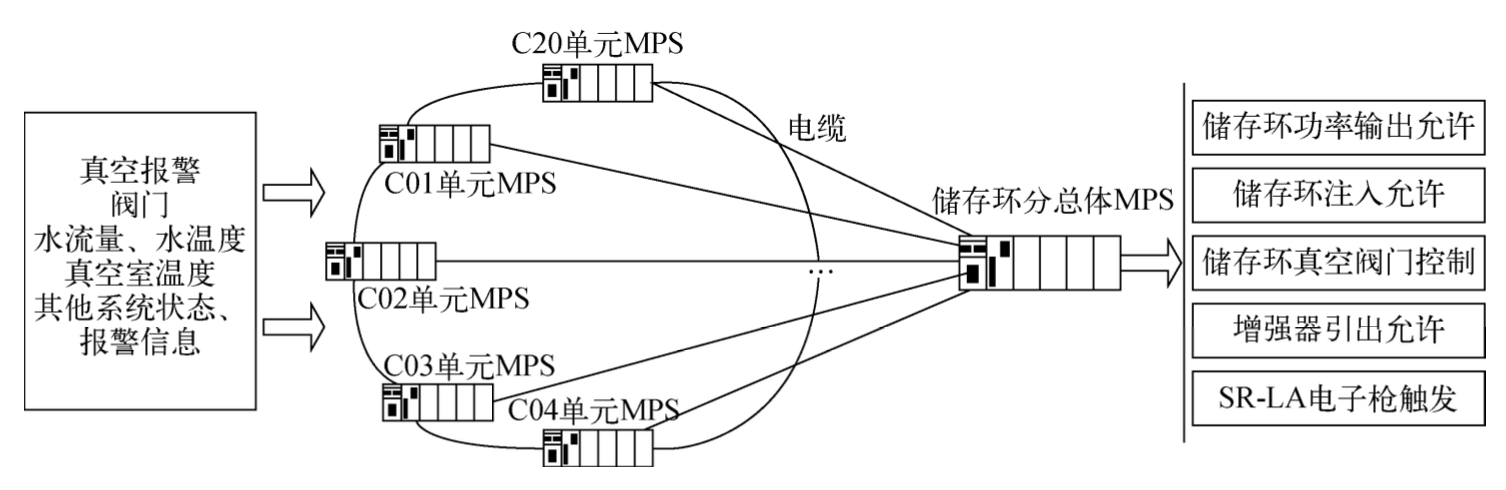
\includegraphics[width=\textwidth]{ssrf-eps-arch-1.png}
	\caption{原有的的储存环机器保护系统结构图}
	\label{fig:ssrf-eps-arch-1}
\end{figure}

上海光源线站工程(二期)为了满足超高磁场二极铁、超导扭摆器、低温波荡器等新增设备的联锁需求,在保证机器保护系统原联锁功能运行正常的情况下,对机器保护系统进行了升级。升级后的机器保护系统架构如图~\ref{fig:ssrf-eps-arch-2}所示,各机器保护系统单元增加了FL-net专用网络通信模块,各单元通过FL-net专用网络连接成菊花链结构,MPS通过FL-net通信解决了联锁系统跨单元通信的问题,满足了低温波荡器真空联锁系统获取相邻单元间阀门信号的联锁需求。经过在线测试,基于FL-net的MPS响应时间小于21ms,满足上海光源加速器运行的需求。

  \begin{figure}[!htb]
	\centering
	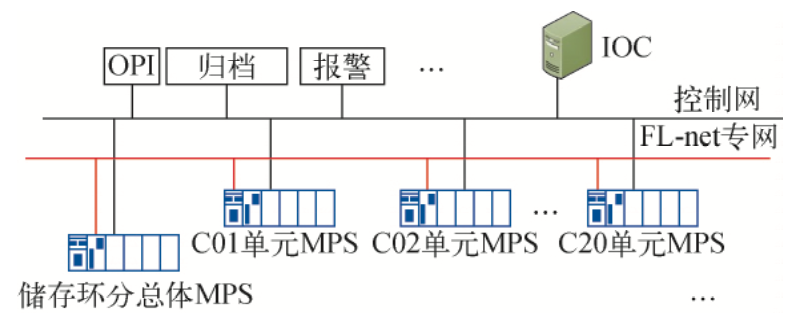
\includegraphics[width=0.85\textwidth]{ssrf-eps-arch-2.png}
	\caption{改造后的储存环机器联锁保护系统结构图}
	\label{fig:ssrf-eps-arch-2}
\end{figure}

\subsubsection{CSNS漂移管直线加速器水冷联锁系统}

中国散裂中子源(China Spallation Neutron Source,CSNS) 是我国在2018年建成的全世界第四台脉冲型散裂中子源,包括一台80MeV负氢漂移管直线加速器(Drift Tube Linac,DTL)、一台1.6GeV快循环质子同步加速器、两条束流输运线、一个靶站以及一期3台中子散射谱仪,CSNS的质子束功率达到10 kW,脉冲重复频率达到25Hz。

  \begin{figure}[!htb]
	\centering
	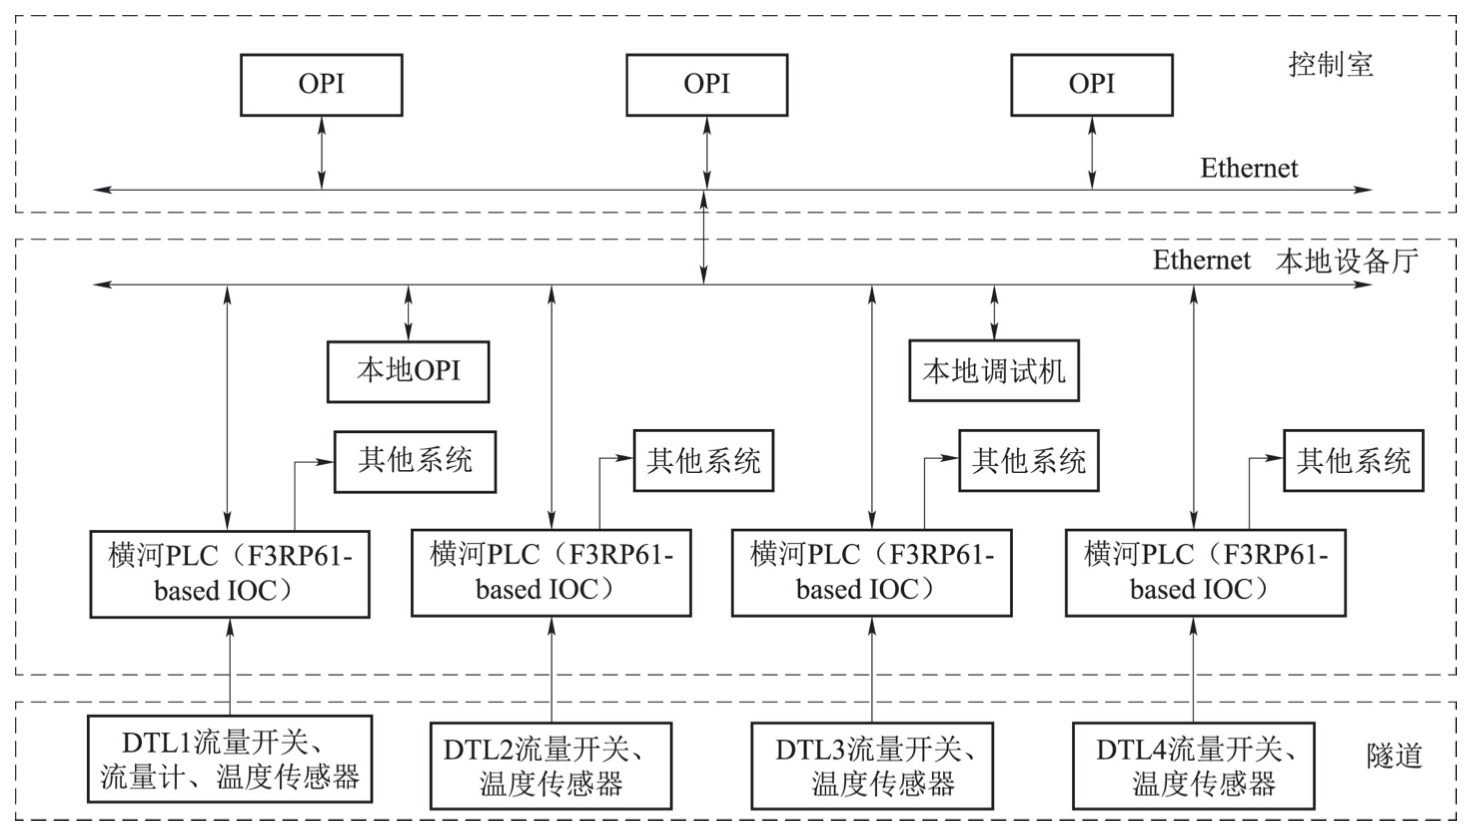
\includegraphics[width=\textwidth]{csns-eps-arch.png}
	\caption{CSNS漂移管直线加速器水冷联锁系统结构图}
	\label{fig:csns-eps-arch}
\end{figure}


DTL水冷联锁系统负责监测DTL的冷却水流量和温度信号,通过控制器逻辑处理后,为磁铁电源和射频系统提供联锁保护信号,系统架构如图~\ref{fig:csns-eps-arch}所示。DTL水冷联锁系统可分为4套子系统,子系统控制器为横河FA-M3 PLC,负责监测冷却水状态信号,经过PLC中CPU模块的联锁处理后,为磁铁电源和射频系统提供保护。EPICS IOC运行在PLC中的嵌入式CPU模块中,负责监控水冷联锁系统的状态\cite{he2017}。



\subsubsection{调研总结}

一般来说,设备保护系统和快保护系统是相对独立的两个系统。其中,大部分加速器装置选择采用PLC作为设备保护系统的联锁控制器,例如上述中的RAON重离子加速器和上海光源,除此之外还有西班牙的ALBA光源等。PLC之间有的采用硬件联锁信号相连,例如改造前的上海光源储存环机器保护系统,上海软X射线自由电子激光装置联锁保护系统\cite{yu2018};有的采用以太网相连,例如ALBA光源PLC之间的通信是基于POWERLINK实现\cite{Alba-eps},升级后的上海光源储存环机器保护系统控制器也增加了FL-net专用网络通信模块\cite{yu2020}。部分加速器装置选择采用FPGA控制器作为设备保护系统的联锁控制器,例如LCLS的联锁控制器,控制器之间采用专用的千兆以太网通信,采用自主设计的通信协议\cite{Norum-2009}。对于FPS的快联锁保护场合,一般采用FPGA控制器来实现,快联锁信号直接连接到联锁控制器中进行处理,例如RAON和J-Parc的快保护系统都采用FPGA控制器来实现快联锁响应\cite{jparc}。

对于HALF设备保护系统,我们计划采用前面研究过的Zynq控制器作为联锁控制器,控制器之间的通信通过千兆POWERLINK实现。同时Zynq控制器也可以作为快保护系统的联锁控制器,只是Zynq控制器之间只能采用联锁信号直接相连的方式。这样,设备保护系统和快保护系统的联锁控制器可以采用同样类型的硬件,为以后的系统运行和维护带来便利。由于本论文主要是研究POWERLINK在加速器装置中的应用研究,所以下文将描述基于POWERLINK的HALF设备保护系统设计。


\section{HALF设备保护系统设计}

\subsection{HALF设备保护系统任务}

作为HALF控制系统的重要组成部分,HALF EPS的任务是在HALF不同的运行模式下保证机器设备的安全。HALF EPS在HALF各分总体、系统间建立联锁保护逻辑,监测的设备状态主要包括真空度、温度、冷却水流量等,在经过系统联锁逻辑判断后,给出禁止电子枪触发、禁止RF功率输出允许、禁止注入等联锁保护信号。HALF EPS遍布整个装置,联锁输入信号分布广泛,数量众多,包括各设备状态信号和来自其他系统的联锁信号,具体可分为以下11类信号:

(1)电子枪状态信号;

(2)真空相关信号;

(3)冷却水状态信号;

(4)磁铁电源状态信号;

(5)微波设备状态信号;

(6)调制器状态信号;

(7)注入系统状态信号;

(8)储存环真空部件温度信号;

(9)插入件状态信号;

(10)来自光束线站的联锁信号;

(11)来自人身安全系统的联锁信号 。


EPS通过给出某些设备的禁止运行信号从而达到保护重要设备的目的,保护措施具体如下:

(1)关闭电子枪驱动激光的光闸;

(2)禁止电子枪触发;

(3)关闭真空阀门;

(4)禁止固态放大器触发;

(5)禁止调制器触发;

(6)切断高频功率输出;

(7)禁止储存环注入。


\subsection{HALF设备保护系统设计原则}

HALF设备保护系统应遵循以下设计原则:

(1) 独立性:设备保护系统直接作用于受保护的设备或系统,其运行不能依赖于其它系统。设备保护系统在设计时要采用专用控制器,控制器之间通过专用网络进行通信。

(2) 失效安全性:当控制器出现故障或联锁信号失联时,该控制器的所有联锁输出信号都将被设置为禁止状态,并实施相应措施切断电子束流,最大程度上保障HALF装置的安全。

(3) 可靠性:设备保护系统应该具有高可靠性,在HALF运行的过程中可以长时间无故障地执行联锁保护任务。一般通过以下技术可以实现系统的高可靠性:硬件冗余设计、系统自检功能、系统Watchdog功能、控制器Heartbeat等。

(4) 实时性:当设备出现故障时,设备保护系统需要在确定的时间内实施保护动作,以及时保护设备安全。
(5) 灵活性:设备保护系统应采用模块化设计并且预留出数量充足的IO 点。这样可以应对系统的需求变化,方便系统扩展。

\subsection{HALF设备保护系统运行模式}

EPS需要接受来自HALF运行管理系统的命令,切换自身的运行模式以满足HALF的运行管理要求。HALF EPS设计了5种运行模式,分别如下:

(1) 停机模式:此模式下HALF处于停机状态,EPS需要确保所有真空阀门均处于关闭状态,并停止所有系统设备的定时触发信号。

(2) 直线加速器调试模式:此模式下仅进行注入器分总体中直线加速器的束流调试,直线加速器的EPS正常开启,旁路掉输运线、储存环EPS的联锁输入信号和来自光束线站的联锁信号。

(3) 注入器调试模式:此模式下仅进行注入器分总体的束流调试,注入器EPS正常开启,旁路掉储存环EPS的联锁输入信号和来自光束线站的联锁信号。

(4) HALF加速器总体调试模式:此模式下进行注入器和储存环的束流调试,注入器EPS和储存环EPS正常开启,旁路来自光束线站的联锁信号。

(5) 运行模式:HALF处于正常的运行状态,此时EPS开启全部联锁保护功能。

\subsection{HALF设备保护系统总体结构}

根据HALF的体系架构,我们可将HALF EPS由上至下分为总体级联锁、分总体级联锁、系统级联锁三个联锁层次,其中,下层系统为上层联锁提供信号,并接收来自上层的联锁保护命令。三个层次的联锁功能具体如下:

(1) 总体级联锁:根据HALF的不同运行模式切换EPS的运行模式;处理HALF各分总体之间的联锁关系,以及接收来自人身安全系统等外部系统的联锁信号,确保整个HALF的运行安全。

(2) 分总体级联锁:负责分总体内各个系统之间设备的联锁保护,保证分总体的安全运行,同时向总体级联锁提供联锁输入信号。

(3) 系统级联锁:负责各系统内部设备的联锁保护,保证分系统运行正常,同时向分总体级联锁系统提供联锁输入信号。

\begin{figure}[!htb]
	\centering
	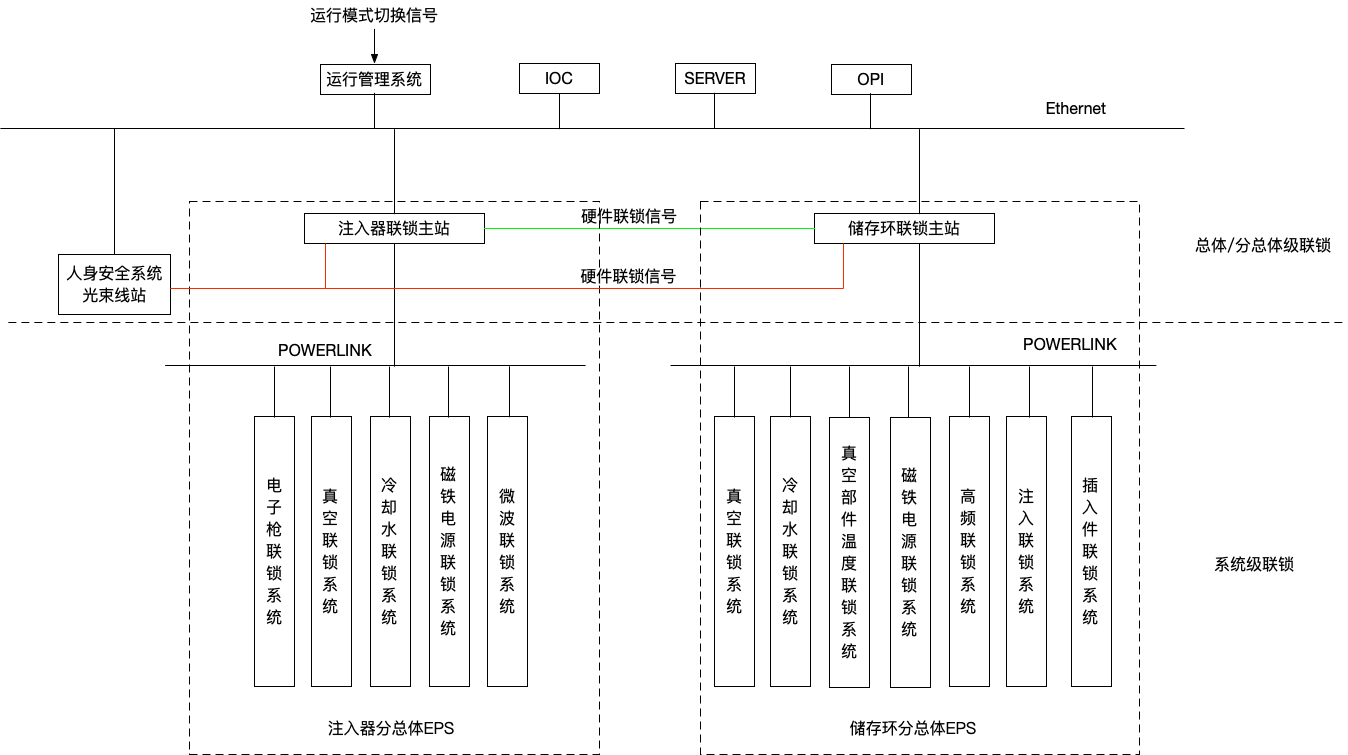
\includegraphics[width=\textwidth]{halfeps-arch.png}
	\caption{HALF EPS总体结构图}
	\label{fig:halfeps-arch}
\end{figure}

根据HALF设备保护系统层次化的结构特点,我们设计了如图~\ref{fig:halfeps-arch}所示的HALF EPS总体结构,可以概括如下:

(1) HALF EPS分为注入器分总体EPS和储存环分总体EPS两部分,分总体EPS负责本分总体范围内的设备安全。按照不同的联锁保护逻辑,我们将注入器分总体EPS分为电子枪联锁系统、真空联锁系统、磁铁电源联锁系统、微波联锁系统、冷却水联锁系统,储存环分总体EPS可分为真空联锁系统、冷却水联锁系统、真空部件温度联锁系统、磁铁电源联锁系统、高频联锁系统、注入联锁系统、插入件联锁系统。

(2) 各分总体EPS基于独立的千兆POWERLINK网络设计,由一个主站控制器和多个从站控制器组成,控制器均采用Zynq控制器。主站控制器负责处理本分总体内各个系统之间的联锁保护关系,从站作为分总体内各系统的EPS控制器,负责收集并处理系统内的设备联锁信号。从站将设备联锁信号通过POWERLINK上传至主站控制器,经过主站控制器的联锁逻辑处理之后,主站通过POWERLINK网络将保护命令传输至相应的从站实施保护。

(3) 注入器EPS主站和储存环EPS主站之间通过硬件信号相连,处理分总体之间的联锁保护关系。

(4) 来自人身安全系统和光束线站的联锁信号采用硬件信号的形式接入分总体EPS主站,通过分总体内相应从站实施保护动作。

(5) EPS主站通过千兆以太网接入HALF控制系统网络中,将设备故障信息和联锁保护信息通过IOC上传至HALF控制系统。同时EPS主站通过控制系统网络接受来自运行管理系统的模式切换命令,切换自身的运行模式以满足HALF的运行管理要求。

\subsection{联锁输入信号的预处理}

HALF设备保护系统运行在不同模式下时,需要对联锁输入信号进行不同的预处理,具体包括旁路、锁存和复位三种处理\cite{chou2008}:

(1) 旁路:设备保护系统处于调试模式时,需要临时解除对部分联锁输入信号的联锁响应,通过将输入信号设置成旁路状态来实现这种需求。旁路的原理:输入信号被设置成旁路状态后,输入信号的实时状态仍可以正常显示,但当输入信号处于报警状态时不会引起系统的联锁保护响应。

(2) 锁存:设备保护系统处于调试模式或者运行模式时,当联锁输入信号处于报警状态时,需要将输入信号设置成锁存状态,保持输入信号的报警状态不变。当输入信号从报警状态恢复到正常状态后,被锁存的输入信号将继续处于故障状态,输入信号引起的联锁输出信号也保持为保护状态,当操作人员解除该输入信号锁存时,才能取消信号的故障状态,从而解除相应的联锁保护。

(3) 复位:当输入信号从故障状态恢复到正常状态时,需要通过复位操作解除信号的锁存状态,复位可分为手动复位和自动复位两种方式。手动复位是操作人员对故障信息进行判断后,通过手动复位操作撤消故障信号的锁存状态;对于部分联锁输入信号,可能需要操作员进行频繁的复位操作,我们在采用自动复位的方式解除联锁信号的锁存状态。

\begin{figure}[!htb]
	\centering
	
\includegraphics[width=0.8\textwidth]{preprocess.png}
	\caption{输入信号预处理流程图}
	\label{fig:preprocess}
\end{figure}

联锁输入信号的预处理流程如图~\ref{fig:preprocess}所示,具体流程如下:

(1) 联锁输入信号首先经过模式旁路和调试旁路的判断,模式旁路指在停机或调试模式下无需对任何联锁输入信号进行处理;调试旁路是指在加速器调试过程中,操作人员对部分输入信号进行的旁路设置,以暂时去掉对这些联锁输入信号的保护响应;

(2) 对联锁输入信号进行锁存处理,对于未被锁存并处于故障状态下的联锁输入信号进行锁存处理;

(3) 对于恢复正常状态的联锁输入信号,通过自动复位或操作人员手动复位的处理对该信号锁存状态进行解除。

(4) 预处理之后的联锁输入信号,再进行联锁逻辑的处理。


下面分别对HALF注入器和储存环分总体EPS的设计进行阐述。

\section{注入器EPS设计}
\label{section:注入器EPS设计}
注入器由直线加速器和输运线组成,直线加速器包括1台光阴极微波电子枪和主加速器,其中光阴极微波电子枪由1台80MW速调管通过波导功分器提供微波功率,主加速器中一共有20个S波段6m等梯度加速段(每个6m等梯度加速段均由2根3m等梯度加速管组合而成),使用20套80MW速调管为主加速器提供微波功率。

注入器分总体EPS的任务是当注入器分总体内各系统设备出现故障或者接收到来自注入器分总体外部的联锁故障信号时,经过注入器联锁主站的联锁逻辑判断后,通过联锁从站实施相应的保护动作。图~\ref{fig:linac-eps-arch}描述了注入器EPS的联锁保护功能。

 \begin{figure}[!htb]
	\centering
	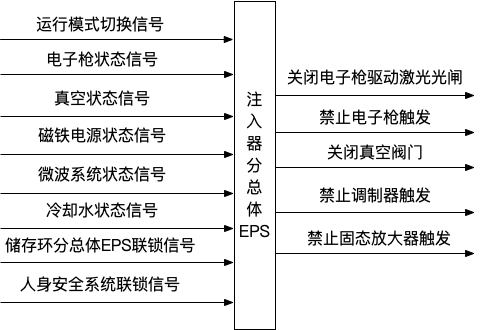
\includegraphics[width=0.75\textwidth]{linac-eps-arch.png}
	\caption{注入器EPS联锁保护功能图}
	\label{fig:linac-eps-arch}
\end{figure}

注入器EPS的输入联锁信号较多,包括运行管理系统的联锁模式切换信号;注入器分总体范围内的真空度信号、冷却水流量和温度信号、电子枪系统状态信号、磁铁电源系统状态信号和微波系统状态信号;来自储存环分总体EPS的联锁信号;来自人身安全系统的联锁信号。注入器EPS提供的保护包括关闭电子枪的驱动激光光闸、关闭真空阀门、禁止电子枪、调制器和固态放大器的时序触发信号。

根据目前HALF注入器的设计参数,注入器分总体EPS可由1台联锁主站和13台联锁从站组成,13台从站按照束流的走向进行部署。直线加速器范围内部署了11台联锁从站,其中电子枪区域内的设备安全由1台从站负责,另外10台从站负责主加速器区域的设备安全,每台从站负责监测连续两个加速段区域内的设备状态信号。输运线范围内的设备较少,部署了2台联锁从站。

联锁主站具有运行模式切换的功能,综合当前运行模式和联锁输入信号,做出相应的逻辑判断,通过相应的从站实施保护。联锁从站负责所在区域内设备的安全,从站的联锁输入信号包括所在区域内的真空度信号、冷却水流量与温度信号以及相应的系统状态信号。联锁输入信号经过从站的联锁逻辑处理后,从站直接实施相应的本地保护,同时将联锁输入信号提供给主站进行联锁逻辑处理。

由于HALF工程还处于预研阶段,注入器各系统的设计细节尚未明确,所以注入器EPS各联锁从站的部署位置以及输入/输出信号数量还未确定,无法描述每个从站的联锁逻辑。下面我们从联锁保护逻辑的角度,以电子枪联锁系统、真空联锁系统和冷却水联锁系统为例,对这些系统相关联锁信号的保护逻辑进行描述。

\subsection{电子枪联锁系统}

电子枪联锁系统的保护任务是对电子枪系统内的联锁信号提供本地保护,同时接收来自主站的保护命令为其他系统的联锁故障信号提供保护。图~\ref{fig:linac-vacuum-eps-global}所示的是电子枪联锁系统的结构图。电子枪联锁系统由电子枪联锁从站负责,输入信号包括电子枪冷却水温度/流量信号、电子枪真空度预警/报警信号、屏蔽间门状态信号、电子枪相应的速调管真空度预警/报警信号和冷却水温度/流量信号、相应的波导真空度报警/预警信号和冷却水温度/流量信号,经过电子枪联锁从站的逻辑判断后,电子枪联锁从站直接实施相应的的保护动作。

\begin{figure}[!htb]
	\centering
	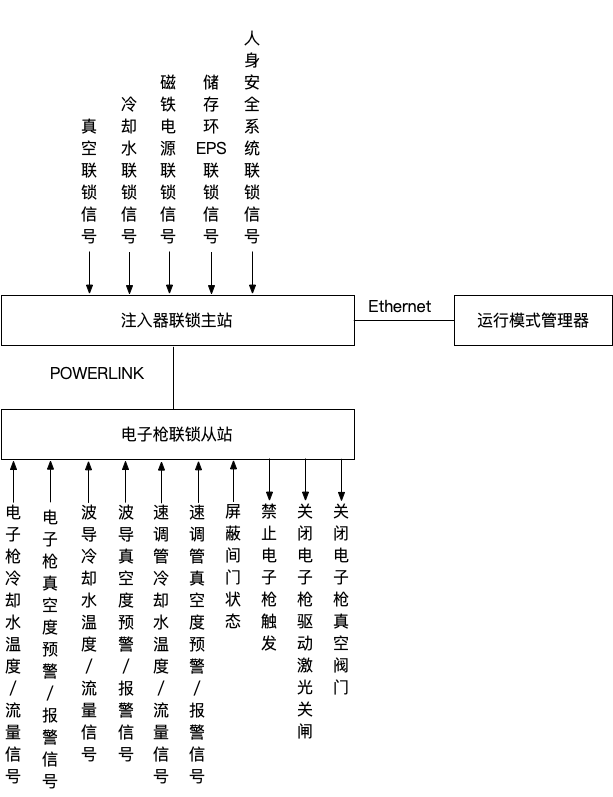
\includegraphics[width=0.7\textwidth]{linac-vacuum-eps-global.png}
	\caption{电子枪系统联锁功能图}
	\label{fig:linac-vacuum-eps-global}
\end{figure}

电子枪联锁系统的本地保护逻辑如下:

(1) 当电子枪系统内以下联锁输入信号故障时,包括屏蔽间门状态信号、电子枪冷却水温度/流量信号和真空度预警信号、电子枪相应的速调管冷却水温度/流量信号和真空度预警信号、相应波导的冷却水温度/流量信号状态和和真空度预警信号,电子枪联锁从站均会关闭驱动激光的光闸、禁止电子枪及其相应的调制器和固态放大器的时序触发信号以停止束流。

(2) 当电子枪、相应的速调管和波导真空度报警时且束流已被打掉,电子枪联锁从站要立即关闭电子枪真空阀门以防止真空泄漏扩散,同时电子枪联锁从站还需要将电子枪真空度故障信号提供给联锁主站,通过相应的从站关闭其余真空阀门。
  		

除了本地保护之外,当其他系统联锁信号出现故障时,注入器联锁主站需要通过电子枪联锁从站实施相应保护,具体的联锁保护逻辑如下:

(1) 当注入器分总统范围内的真空度信号出现故障时,电子枪联锁从站会关闭电子枪真空阀门以防止真空泄漏扩散,同时关闭驱动激光的光闸和切断电子枪的时序触发信号以停止束流。

(2) 当注入器分总体内冷却水温度/流量信号、磁铁电源状态信号、来自储存环分总体和人身安全系统的联锁信号出现故障时,电子枪联锁从站实施关闭驱动激光的光闸和切断电子枪时序触发信号的保护动作。
  		


\subsection{真空联锁系统}

真空联锁系统的任务是对注入器范围内的真空度联锁信号提供相应的保护措施,联锁输入信号包括真空度预警信号和报警信号,其中真空度预警值小于真空度报警值,图~\ref{fig:linac-vacuum-eps}所示的是真空联锁系统结构图,联锁输入信号具体包括电子枪区域内的电子枪、波导管、速调管的真空度预警/报警信号;主加速器区域内20个加速段的真空度预警/报警信号、40根波导管的真空度预警/报警信号、20台速调管的真空度预警/报警信号;输运线真空度预警/报警信号。真空联锁系统的输出保护信号包括禁止电子枪、21台固态放大器和21台调制器的时序触发信号和关闭注入器范围内相应的真空阀门,其中注入器范围内的真空阀门共22台,分别位于电子枪出口处、每个加速段出口处和输运线出口处\cite{wei2014}。

\begin{figure}[!htb]
	\centering
	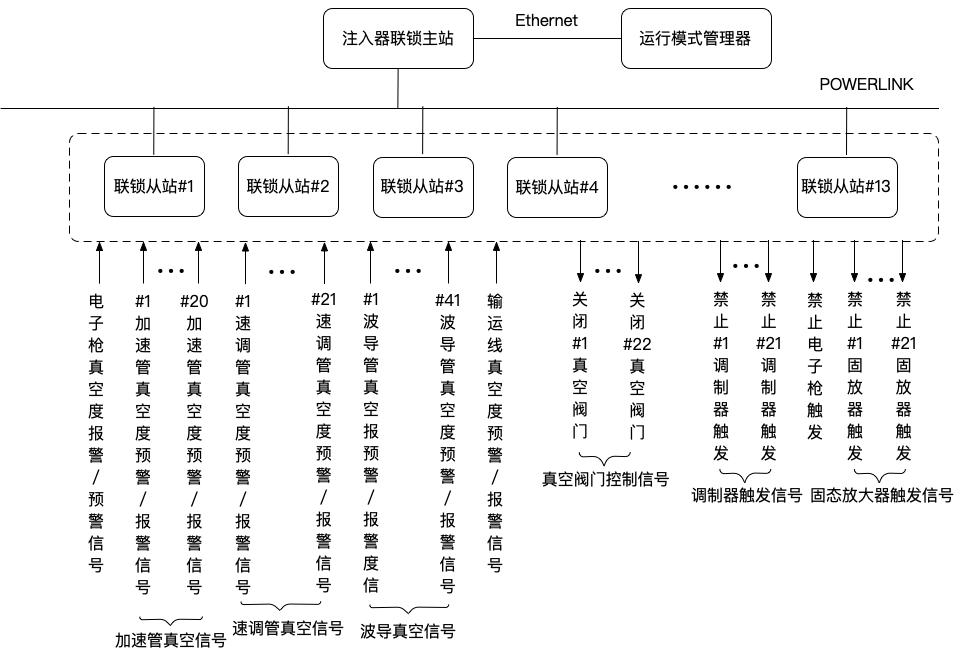
\includegraphics[width=1.05\textwidth]{linac-vacuum-eps.png}
	\caption{真空联锁系统结构图}
	\label{fig:linac-vacuum-eps}
\end{figure}

电子枪的真空联锁保护逻辑已在电子枪联锁系统中进行了描述,其余设备的真空联锁保护逻辑具体如下:

(1) 加速段真空保护:当加速段的真空度处于预警值和报警值之间时,负责监测此加速段的从站直接切断相应的固态放大器和调制器时序触发信号,同时将预警信息上传到联锁主站,通过电子枪从站实施关闭激光光闸、切断电子枪和电子枪对应的固态放大器和调制器时序触发信号。当加速段真空度大于报警值且束流已被打掉后,负责监测此加速段的从站直接关闭此区域的真空阀门,同时将报警信息上传到联锁主站,主站通过相应的从站关闭相应的真空阀门以防止真空进一步泄漏。

(2) 速调管真空保护:当速调管的真空度处于预警值和报警值之间时,负责监测此速调管的从站直接切断相应的固态放大器和调制器时序触发信号,同时将预警信息上传到联锁主站,通过电子枪从站实施关闭激光光闸、切断电子枪和电子枪对应的固态放大器和调制器时序触发信号。当速调管真空度大于报警值且束流已被打掉后,负责监测此速调管的从站直接该区域的真空阀门,同时将报警信息上传到联锁主站,主站通过相应的从站关闭相应的真空阀门以防止真空进一步泄漏。

(3) 波导真空保护:当波导的真空度处于预警值和报警值之间时,负责监测此波导的从站直接切断相应的固态放大器和调制器时序触发信号,同时将预警信息上传到联锁主站,通过电子枪从站实施关闭激光光闸、切断电子枪和电子枪对应的固态放大器和调制器时序触发信号。当波导真空度大于报警值且束流已被打掉后,负责监测此速调管的从站直接关闭该区域的真空阀门,同时将报警信息上传到联锁主站,主站通过相应的从站关闭相应的真空阀门以防止真空进一步泄漏。

(4) 当输运线的真空度处于预警值和报警值之间时,输运线从站将预警信息上传到联锁主站,通过电子枪从站实施关闭激光光闸、切断电子枪和电子枪对应的固态放大器和调制器时序触发信号。注入器联锁主站还会通过将故障信息通过硬件信号传输给储存环联锁主站,储存环EPS实施禁止高频功率输出和禁止储存环注入的保护动作。当输运线真空度大于报警值且束流已被打掉后,负责监测此输运线的从站直接关闭该区域的真空阀门,同时将报警信息上传到联锁主站,主站通过相应的从站关闭相应的真空阀门以防止真空进一步泄漏。

\subsection{冷却水联锁系统}


磁铁线圈与磁铁电源的冷却水温度/流量信号直接与其磁铁电源相连,综合成为一路电源状态信号输入到相应联锁从站,


冷却水联锁系统的任务是对注入器范围内的冷却水温度/流量信号提供相应的保护措施。冷却水联锁系统的结构如图~\ref{fig:linac-coolingwater-eps}所示,冷却水联锁系统的输入信号是注入器各区域的冷却水温度/流量信号,具体包括电子枪及其速调管和波导的冷却水温度/流量信号、主加速器区域内40根加速管的冷却水温度/流量信号、40根波导管的冷却水温度/流量信号和20台速调管的冷却水温度/流量信号,除此以外磁铁线圈与磁铁电源的冷却水温度/流量信号直接与其磁铁电源相连,综合成为一路电源状态信号输入到相应联锁从站。注入器电源分为直线段和输运线段2个单元,直线段预估包括中功率电源3台、小功率电源 84台,输运线段预估包括大中功率电源11台、小功率电源89台,注入器的磁铁电源状态信号一共是187路\cite{sun2018}。


冷却水EPS的输出保护信号包括禁止电子枪、22台固态放大器和22台调制器的时序触发信号。

\begin{figure}[!htb]
	\centering
	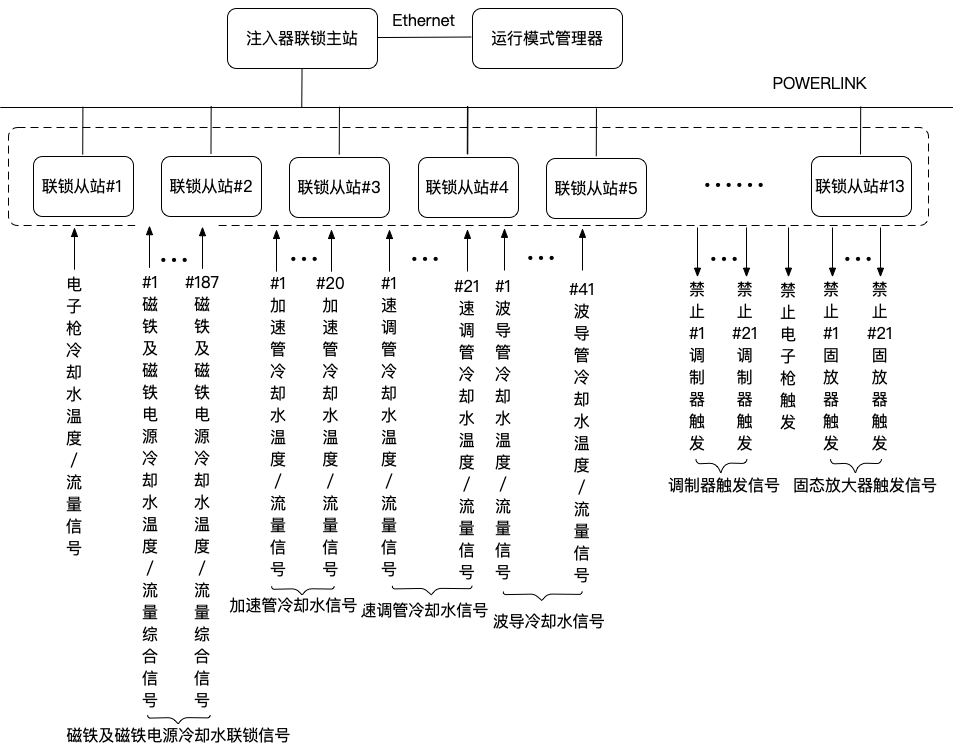
\includegraphics[width=1.05\textwidth]{linac-coolingwater-eps.png}
	\caption{冷却水EPS联锁保护功能图}
	\label{fig:linac-coolingwater-eps}
\end{figure}

电子枪冷却水联锁保护逻辑已在电子枪联锁系统中进行了描述,其余设备的冷却水联锁保护逻辑具体如下:

(1) 磁铁及磁铁电源磁铁的冷却水联锁保护:当磁铁电源状态信号信号出现故障时,经过联锁主站逻辑处理后,通过电子枪从站实施关闭驱动激光的光闸和切断电子枪、调制器和固态放大器时序触发信号的保护动作。

(2) 加速管冷却水联锁保护:当加速管的冷却水温度/流量信号出现故障时,负责此区域的从站直接切断此加速管对应的固态放大器和调制器时序触发信号;同时将故障信息上传到联锁主站,主站通过电子枪从站关闭驱动激光的光闸和切断电子枪、调制器和固态放大器时序触发信号。

(3) 速调管冷却水保护:当速调管的冷却水温度/流量信号出现故障时,负责此区域的从站直接切断此速调管对应的固态放大器和调制器时序触发信号。

(4) 波导冷却水保护:当波导的冷却水温度/流量信号出现故障时,负责此区域的从站直接切断此波导对应的固态放大器和调制器时序触发信号。

\subsection{注入器分总体EPS联锁信号总结}

根据最新的HALF设计参数,我们对注入器EPS分总体的联锁信号进行了初步统计,各系统联锁信号数量如表~\ref{table:4.2}所示。

\begin{table}[!hbt]
  \centering
  \caption{注入器EPS的联锁信号数量统计表}
  \label{table:4.2} 
  \begin{center}
  \begin{tabular}{cccccc}
    \toprule

     系统名称&联锁输入信号&联锁保护信号\\
    \midrule
    电子枪联锁系统& 1& 2 \\
    
    真空联锁系统  & 168 & 22 \\
    
    磁铁电源联锁系统 &187 & 0\\
    
    微波联锁系统 & 21 & 42 \\
    
    冷却水联锁系统  & 166& 0\\

    储存环分总体EPS & 1& 0\\
    
    人身安全系统& 1& 0\\

    总计&545& 66\\

    \bottomrule
  \end{tabular}
\end{center}
\end{table}


\subsection{注入器设备保护系统实时性能评估}

根据注入器分总体设备保护系统的设计方案,我们可以将第~\ref{section:全站FPGA方案的系统设计与开发}节中全站FPGA方案的测试系统作为注入器分总体EPS的原型系统,但是由于原型系统的从站数量仅为5台,无法满足注入器设备保护系统13台联锁从站的规模。下面我们将根据注入器设备保护系统的设计规模和具体联锁信号数量,采用理论计算和网络模拟两种方法对注入器设备保护系统的实时性能进行评估。

\subsubsection{理论计算}

我们首先对注入器设备保护系统的通信周期进行分析计算。通信周期由等时同步阶段和空闲阶段组成,等时同步阶段的时长公式为~\ref{equation27},其中$T_{sync}$为SoC数据帧同步各从站的时间,$T_{sync}$由SoC数据帧的传输时间和各从站接收并处理SoC帧的时间组成,根据第~\ref{section:全站FPGA方案通信周期的理论计算}节中对同步阶段的理论分析,$T_{sync}$的最大值一般不超过1$\mu$s。

\begin{equation}
\label{equation27}
T_{ip}=T_{sync}+T_{poll}
\end{equation}

轮询阶段时长$T_{poll}$按照公式~\ref{equation28}来计算,其中$sum_{i=1}^{13}(T_{F(PRes)}^{i}$+$T_{F(PReq)}^{i})$为13个联锁从站的PReq/PRes数据帧的传输时间之和。注入器设备保护系统系统中所有PReq/PRes帧的总数据量可通过公式~\ref{equation29}进行计算,总数据量($sum_{i=1}^{13}(DataSize_{PReq}^{i}+DataSize_{PRes}^{i})$)由PReq/PRes数据帧的帧头帧尾总数据量($DataSize_{total}^{frame}$)和PReq/PRes数据帧的应用层总数据量($DataSize_{total}^{user\_data}$)组成。根据第~\ref{subsection:POWERLINK协议的网络模型}节中对POWERLINK数据帧结构的分析,PReq数据帧和PRes数据帧的帧头帧尾大小($DataSize_{format}^{PReq}$,$DataSize_{format}^{PReq}$)均为31Byte,根据公式~\ref{equation30},可得13个联锁从站的PReq/PRes数据帧的帧头帧尾总数据量($DataSize_{total}^{format}$)等于806Byte。

PReq和PRes数据帧中的应用层数据分别对应于该从站的输出信号和输入信号,考虑到与联锁信号相关的锁存、旁路和复位预处理状态信号也需要通过PReq/PRes数据帧参与通信,我们按照一个输入/输出信号的相关数据大小为1Byte来进行计算,根据公式~\ref{equation31},PReq和PRes数据帧中的应用层数据即等于系统联锁信号的总数量。
根据表~\ref{table:4.2}的统计结果,注入器设备保护系统中联锁信号的总数量为611,考虑到保护设备的状态回读信号,我们在计算时将联锁信号数量翻倍,即按照1222个总联锁信号数量来进行计算。


我们将$DataSize_{total}^{format\_data}$和$Datasize_{total}^{user\_data}$的数值代入公式~\ref{equation29},得到系统中所有PReq/PRes数据帧的总大小为2028Byte,按照千兆以太网的速率进行数据传输,可计算出PReq/PRes数据帧传输时间之和($\sum_{i=1}^{13}(T_{F(PReq)}^{i}+T_{F(PRes)}^{i})$)为20.280$\mu$s。

\begin{equation}
\begin{split}
\label{equation28}
T_{poll}=\sum_{i=1}^{13}(T_{F(PReq)}^{i}+T_{F(PRes)}^{i})+T_{net}^{line}\\
\end{split}
\end{equation}

\begin{equation}
\begin{split}
\label{equation29}
sum_{i=1}^{13}(DataSize_{PReq}^{i}+DataSize_{PRes}^{i}) = DataSize_{total}^{format}+DataSize_{total}^{user\_data}\\
\end{split}
\end{equation}


\begin{equation}
\begin{split}
\label{equation30}
DataSize_{total}^{format} = 13(DataSize_{format}^{PReq}+DataSize_{format}^{PRes})\\
\end{split}
\end{equation}


\begin{equation}
\begin{split}
\label{equation31}
D_{total}^{user\_data} = sum_{i=1}^{13}(D_{InputSignal}^{i}+D_{outputSignal}^{i})\\
\end{split}
\end{equation}


公式~\ref{equation28}中的$T_{net}^{line}$为注入器设备保护系统的网络组件延时,各联锁从站按照线型拓扑结构相连,$T_{net}^{line}$可按照公式~\ref{equation32}进行计算,其中$T_{c}$为相邻两节点之间网线的传输延时,注入器260m长度,这里假定各联锁从站按照等距离部署,相邻从站之间的距离为22m,按照5ns/m的传输延时计算,$T_{c}$为0.110$\mu$s。 $T_{hub}$ 、$T_{r-cn}$ 、$T_{r-mn}$参数根据第~\ref{section:全站FPGA方案通信周期的理论计算}节中系统的实测结果,分别为1.717$\mu$s、0.925$\mu$s和0.661$\mu$s,代入公式~\ref{equation32},可得$T_{net}^{line}$为166.075$\mu$s。

\begin{equation}
\begin{split}
\label{equation32}
T_{net}^{line}&=\sum_{i=1}^{13}[2iT_{c}+(2i-1)T_{hub}+T_{r-cn}]+nT_{r-mn}\\
\end{split}
\end{equation}

将$T_{net}^{line}$和$\sum_{i=1}^{13}(T_{F(PReq)}^{i}+T_{F(PRes)}^{i})$代入公式~\ref{equation28},可得轮询阶段时长$T_{poll}$为186.355$\mu$s,加上同步阶段的时长$T_{sync}$,则等时同步阶段的时长$T_{ip}$为187.355$\mu$s。

考虑到空闲阶段时长为定值,为传输最大异步数据预留的时间,根据第~\ref{section:全站FPGA方案通信周期的理论计算}节中系统的实测结果为12.920$\mu$s,可得注入器设备保护系统通信周期为199.275$\mu$s。


根据第~\ref{subsection:系统性能测试与分析}节中对系统响应时间的分析,耗时最长的响应过程为联锁输入信号从1号从站输入,经过主站处理后,通过13号从站输出保护动作,此过程跨越3个周期,考虑到输入信号的通信等待时间和从站数字隔离器5$\mu$s的信号处理时间,注入器设备保护系统的最长响应时间约为802.100$\mu$s。


\subsubsection{网络模拟}

基于OMNeT++仿真平台,我们对注入器设备保护系统进行了建模,模型如图~\ref{fig:13node-model-omnet}所示。

\begin{figure}[!htb]
  \centering
  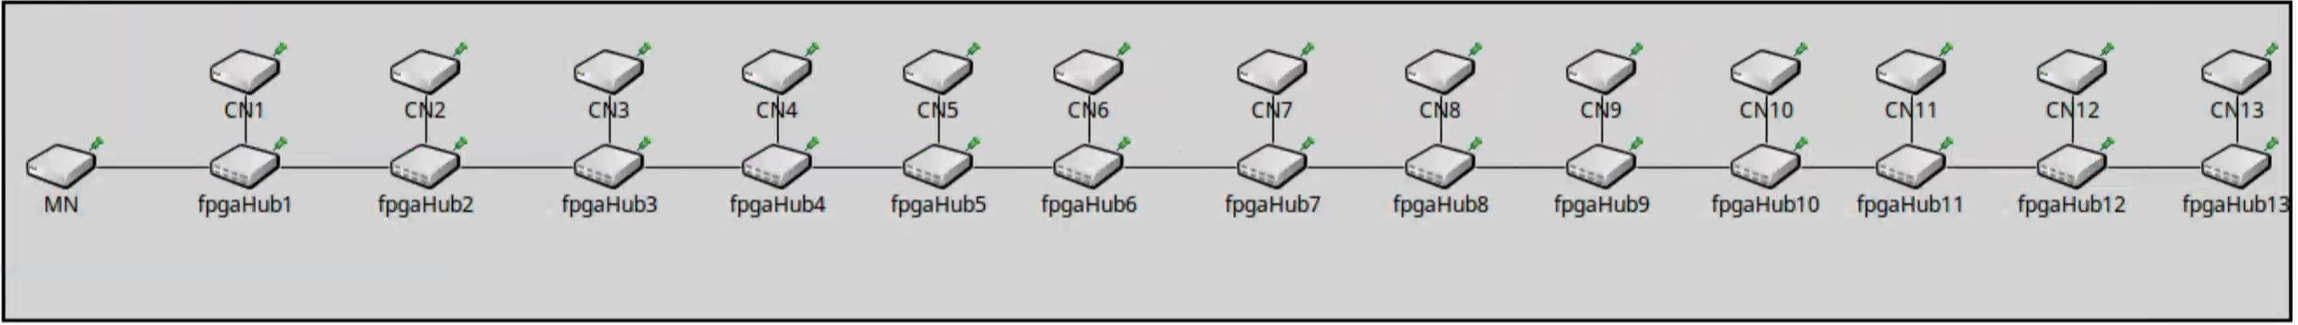
\includegraphics[width=\textwidth]{13node-model-omnet.png}
  \caption{注入器设备保护系统模型}
  \label{fig:13node-model-omnet}
\end{figure}

根据第~\ref{section:全站FPGA方案通信周期的理论计算}对通信周期的理论分析,各联锁从站被分配的通信时隙($T_{cn-slot}^{i}$)可通过公式~\ref{equation33}和公式~\ref{equation34}计算得到,其中各从站的PReq数据帧和PRes数据帧的传输时间$T_{F(PReq)}^{i}$和$T_{F(PRes)}^{i}$跟该从站的输入和输出信号数量有关,我们根据第~\ref{section:注入器EPS设计}节中注入器设备保护系统各从站的部署情况,可以对各从站的联锁信号数量进行估算,考虑到保护的回读状态信号,这里同样将联锁信号数量翻倍来进行计算。$T_{hub}$ 、$T_{r-cn}$ 、$T_{r-mn}$参数按照第~\ref{section:全站FPGA方案通信周期的理论计算}节中系统的实测结果,分别为0.661$\mu$s、0.925$\mu$s和1.717$\mu$s,根据公式~\ref{equation34}可以计算出各联锁从站被配置的通信时隙(PResTimeout)。

\begin{equation}
\label{equation33}
T_{rtd}^{i}=2iT_{c}+(2i-1)T_{hub}+T_{r-cn}
\end{equation}

\begin{equation}
\label{equation34}
T_{cn-slot}^{i}=T_{F(PReq)}^{i}+T_{F(PRes)}^{i}+T_{rtd}^{i}+T_{r-mn}
\end{equation}

各从站具体配置如下所示,其中PResTimeout为各联锁从站的通信时隙,PReqActPayload为各从站的输出信号大小。

\begin{lstlisting}
<Nodes>
  <Node NodeId="1" PResTimeout="6129ns" PReqActPayload="5byte" />
  <Node NodeId="2" PResTimeout="6998ns" PReqActPayload="6byte" />
  <Node NodeId="3" PResTimeout="8538ns" PReqActPayload="6byte" />
  <Node NodeId="4" PResTimeout="10078ns" PReqActPayload="6byte" />
  <Node NodeId="5" PResTimeout="11618ns" PReqActPayload="6byte" />
  <Node NodeId="6" PResTimeout="13158ns" PReqActPayload="6byte" />
  <Node NodeId="7" PResTimeout="14698ns" PReqActPayload="6byte" />
  <Node NodeId="8" PResTimeout="16238ns" PReqActPayload="6byte" />
  <Node NodeId="9" PResTimeout="17778ns" PReqActPayload="6byte" />
  <Node NodeId="10" PResTimeout="19318ns" PReqActPayload="6byte" />
  <Node NodeId="11" PResTimeout="20858ns" PReqActPayload="6byte" />
  <Node NodeId="12" PResTimeout="24749ns" PReqActPayload="1byte" />
  <Node NodeId="13" PResTimeout="26289ns" PReqActPayload="1yte" />
</Nodes>
\end{lstlisting}

模拟过程持续了大约1000个POWERLINK通信周期。等时同步阶段的概率密度分布绘制在图~\ref{fig:iso-time-density-13cn-model}中,该图表明注入器设备保护系统轮询平均时长为184.376$\mu$s。考虑到同步阶段时长$T_{sync}$最大为1$\mu$s和12.920$\mu$s的空闲时长,可得注入器设备保护系统通信周期为198.296$\mu$s。考虑到输入信号的通信等待时间和从站数字隔离器5$\mu$s的信号处理时间,注入器设备保护系统的最长响应时间约为798.184$\mu$s。

\begin{figure}[!htb]
  \centering
  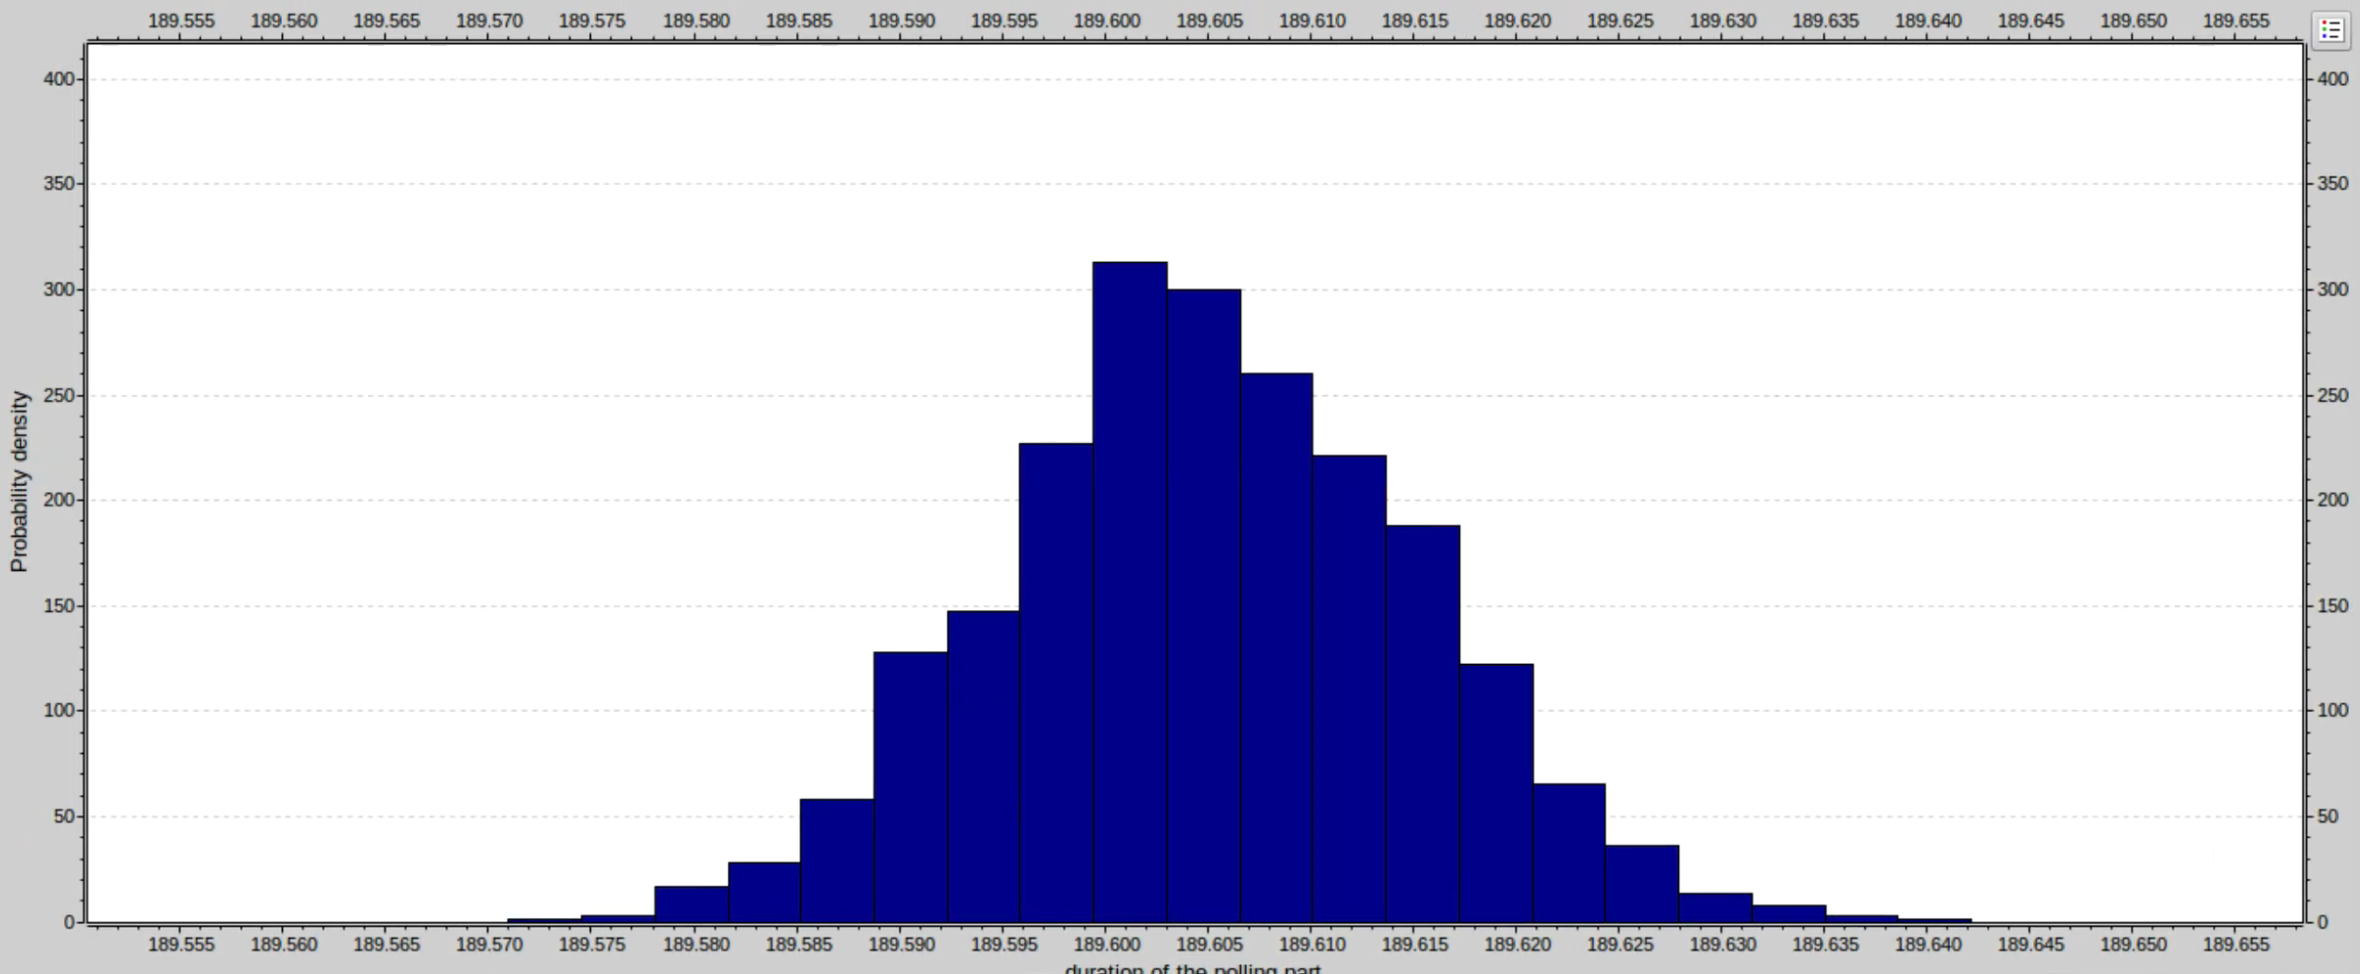
\includegraphics[width=\textwidth]{iso-time-density-13cn-model.png}
  \caption{注入器设备保护系统模型轮询阶段时长的概率密度分布}
  \label{fig:iso-time-density-13cn-model}
\end{figure}

\subsubsection{小结}

我们通过理论计算和仿真模拟的方法两种方法对注入器设备保护系统的实时性能进行了估算,两种方法的计算结果比较相近,通信周期的估算结果分别为199.275$\mu$s和198.296$\mu$s,最大响应时间的的估算结果分别为802.100$\mu$s和798.184$\mu$s,通过理论计算和仿真模拟的方法两种方法得到的结果较接近,均完全满足设备保护系统响应时间10ms响应时间的需求。



\section{储存环分总体EPS设计}

HALF储存环由20个全同的多弯铁消色散结构(MBA)的聚焦单元组成,每个单元长度为24m,可提供一个5.5m的长直线节和一个2.2m的中直线节。储存环周长为480m,可以提供20个长直线节和20个中直线节,除了两个直线节分别安装注入系统和高频系统外,其中至少35个直线节可用于安装插入元件,目前一期HALF工程计划建设10条插入件光束线。

储存环分总体EPS的任务是当储存环分总体内各系统设备出现故障或者接收到来自储存环分总体外部的联锁故障信号时,经过储存环联锁主站的逻辑处理后,通过联锁从站实施相应的保护动作。图~\ref{fig:ring-interlock-signal}描述了储存环分总体EPS的联锁保护功能。

\begin{figure}[!htb]
	\centering
	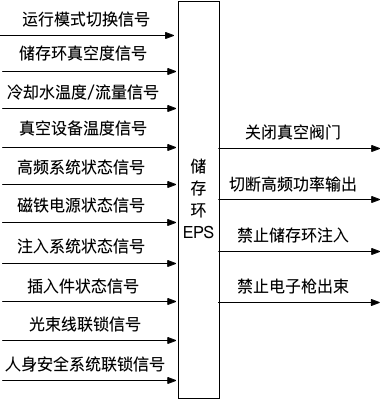
\includegraphics[width=0.7\textwidth]{ring-interlock-signal.png}
	\caption{储存环EPS联锁保护功能图}
	\label{fig:ring-interlock-signal}
\end{figure}

储存环EPS的输入联锁信号较多,包括来自运行管理系统的联锁模式切换信号;储存环分总体范围内的真空度信号、冷却水温度/流量信号、真空部件温度信号、磁铁电源状态信号、高频系统状态信号、注入系统状态信号、插入件系统状态信号;来自光束线站和人身安全系统的联锁信号。储存环EPS提供的保护措施具体如下:关闭储存环范围内的真空阀门、禁止高频功率输出、禁止储存环注入和通过注入器联锁主站停止电子枪出束。

根据目前HALF储存环的设计参数,储存环分总体EPS可由1台联锁主站和20台联锁从站组成,20台从站按照20个MBA单元的位置部署在整个储存环分总体范围内。联锁主站具有运行模式切换的功能,综合当前运行模式和联锁输入信号,做出相应的逻辑判断,通过相应的从站实施保护措施。20台联锁从站负责所在区域内设备的安全,从站的联锁输入信号包括所在区域内的真空度信号、冷却水流量/温度信号、真空设备温度信号以及相应的系统状态信号。联锁输入信号经过从站的联锁逻辑处理后,从站直接实施相应的本地保护,同时将联锁输入信号提供给主站进行逻辑处理。

由于HALF工程还处于预研阶段,储存环各系统的设计细节尚未明确,所以储存环EPS各联锁从站的部署位置以及输入/输出信号数量还未确定,无法描述每个从站的联锁逻辑。下面我们从联锁保护逻辑的角度,以真空联锁系统、冷却水联锁系统、真空部件温度联锁系统、高频联锁系统和注入联锁系统为例,对这些系统相关联锁信号的保护逻辑进行描述。

\subsection{真空联锁系统}

真空联锁系统的输入信号是储存环范围内的真空度信号,包括真空度预警信号和报警信号,其中真空度预警值小于真空度报警值。全环一共120个真空度联锁输入信号,由20个联锁从站负责,每个从站负责相应区域内的3个真空度预警信号和3个真空度报警信号,这里暂时不考虑光束线前端区和光束线站的真空度联锁信号,光束线的真空保护由光束线联锁保护系统负责。联锁从站的输出信号是真空阀门控制信号,全环共20台真空阀门,分别位于相邻两个MBA单元之间。

图~\ref{fig:ring-eps-vacuum}所示的是真空联锁系统结构图。

\begin{figure}[!htb]
	\centering
	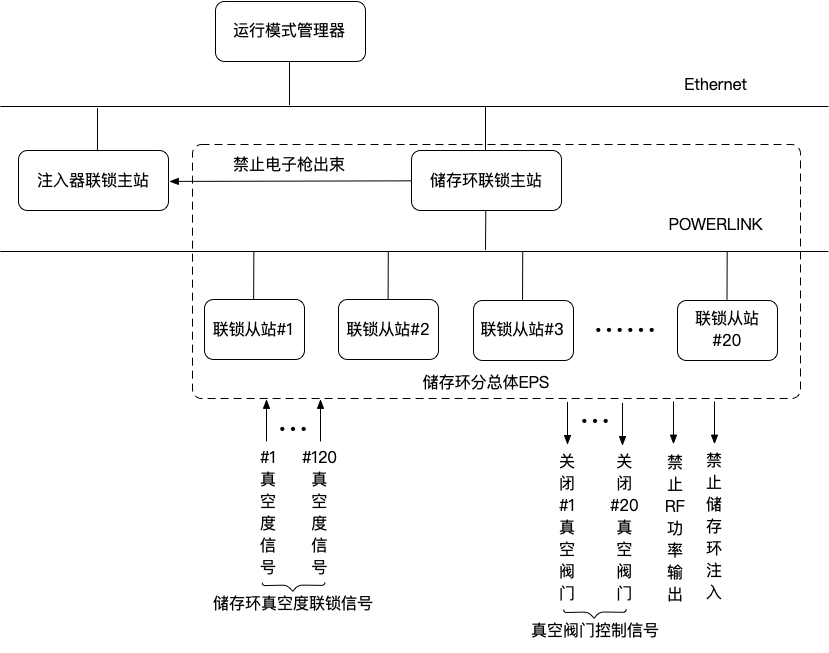
\includegraphics[width=\textwidth]{ring-eps-vacuum.png}
	\caption{真空联锁系统结构图}
	\label{fig:ring-eps-vacuum}
\end{figure}

对于真空度预警信号和真空度报警信号,真空联锁系统的具体保护措施如下:

(1) 当储存环真空度处于预警值和报警值之间时,负责此区域的联锁从站将故障信息上传到联锁主站,主站通过相应的从站实施禁止高频功率输出和储存环注入的保护动作,同时将联锁故障信号传输给注入器联锁主站,通过电子枪从站实施关闭激光光闸和切断电子枪时序触发信号的保护动作。

(2) 当储存环真空度高于报警值且束流已被打掉后,负责监测此真空度信号的从站直接关闭此单元的真空阀门,同时将报警信息上传到联锁主站,主站通过相应的从站关闭相应的真空阀门以防止真空进一步泄漏。

\subsection{冷却水联锁系统}

冷却水联锁系统的输入信号是储存环各区域的冷却水温度/流量信号,具体如下:

(1)真空部件的冷却水温度/流量信号:每个联锁从站负责相应区域的弯段、光子吸收器和波纹管共24个冷却水温度/流量信号,全环共480个真空部件的冷却水温度/流量信号;

(2) 磁铁及磁铁电源的冷却水温度/流量信号:储存环磁铁电源系统设计为20个单元,每个单元磁铁包括6块纵向梯度二极铁、4块二四极组合铁、16块四极铁、6块六极铁、2台八极铁和12块校正铁,其中四极铁和校正铁均单独供电,其他磁铁是分成若干组串联供电。各单元中的磁铁线圈与磁铁电源的冷却水温度/流量信号直接与其磁铁电源相连,综合成为一路电源状态信号输入到相应联锁从站,每个从站的联锁输入信号具体包括16路四级铁电源状态信号、12路校正铁电源状态信号、1路二级铁电源状态信号、1路六级铁电源状态信号和1路八级铁电源状态信号,共31路联锁输入信号,全环共620路磁铁电源状态信号。

(3) 10个插入件的冷却水温度/流量信号,由相应的联锁从站负责。

\begin{figure}[!htb]
	\centering
	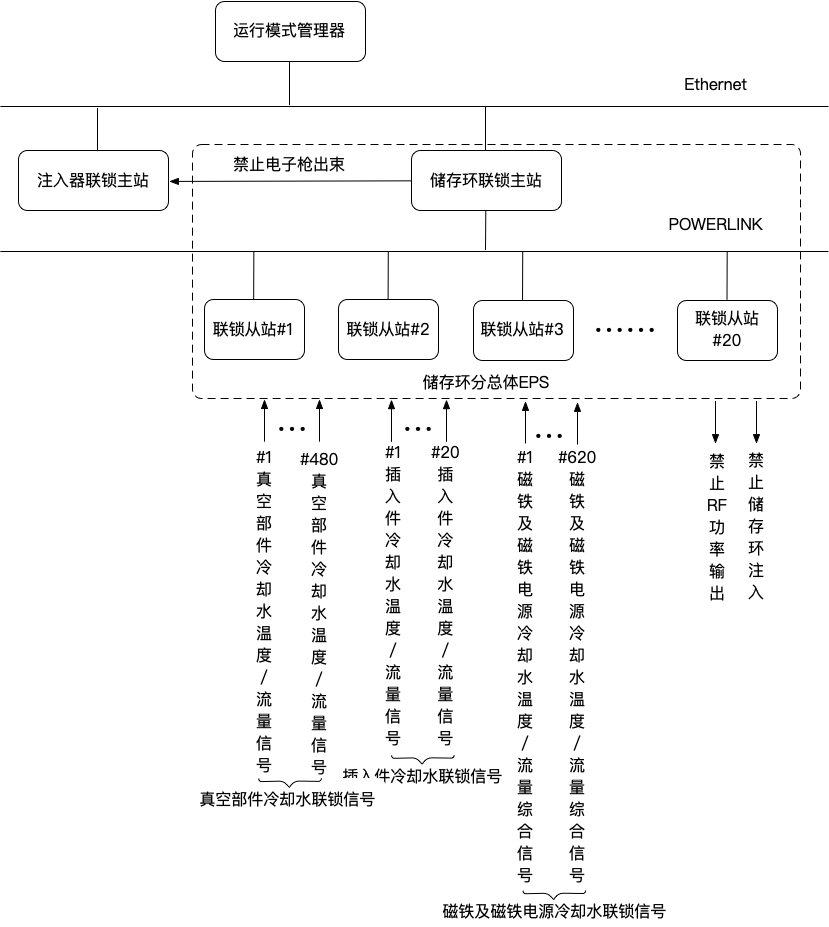
\includegraphics[width=0.95\textwidth]{ring-water-eps.png}
	\caption{冷却水联锁系统结构图}
	\label{fig:ring-water-eps}
\end{figure}

图~\ref{fig:ring-water-eps}所示的是冷却水联锁系统功能图,冷却水联锁系统的具体联锁保护逻辑如下:

(1) 真空部件冷却水联锁保护:当真空盒、光子吸收器和波纹管等真空部件的冷却水温度高于阈值,或这些这些真空部件的冷却水流量低于阈值时,相应的联锁从站将故障信息提供给联锁主站,经过主站的逻辑处理后,通过高频系统从站切断高频功率输出;通过注入系统联锁从站实施禁止储存环注入的保护动作;同时将联锁故障信号传输给注入器联锁主站,通过电子枪从站关闭激光光闸并切断电子枪、调制器和固态放大器时序触发信号。

(2) 高频腔冷却水联锁保护:当高频腔冷却水温度/流量信号出现故障时,高频腔联锁从站实施切断高频功率输出的本地保护措施;同时从站将故障信息上传到联锁主站,经过联锁主站逻辑处理后,通过注入系统联锁从站实施禁止储存环注入的保护动作;同时将联锁故障信号传输给注入器联锁主站,通过电子枪从站关闭激光光闸并切断电子枪、调制器和固态放大器时序触发信号。

(3) 磁铁冷却水联锁保护:当磁铁线圈的冷却水温度/流量信号出现故障时,相应的联锁从站将故障信息提供给联锁主站,经过主站逻辑处理后,通过高频系统从站切断高频功率输出;通过注入系统联锁从站实施禁止储存环注入的保护动作;同时将联锁故障信号传输给注入器联锁主站,通过电子枪从站关闭激光光闸并切断电子枪、调制器和固态放大器时序触发信号。

(4) 插入件冷却水联锁保护:当插入件的冷却水温度/流量信号出现故障时,相应的联锁从站将故障信息提供给联锁主站,经过联锁主站逻辑处理后,通过高频系统从站切断高频功率输出;通过注入系统联锁从站实施禁止储存环注入的保护动作;同时将联锁故障信号传输给注入器联锁主站,通过电子枪从站关闭激光光闸并切断电子枪、调制器和固态放大器时序触发信号。

\subsection{真空部件温度联锁系统}

\begin{figure}[!htb]
	\centering
	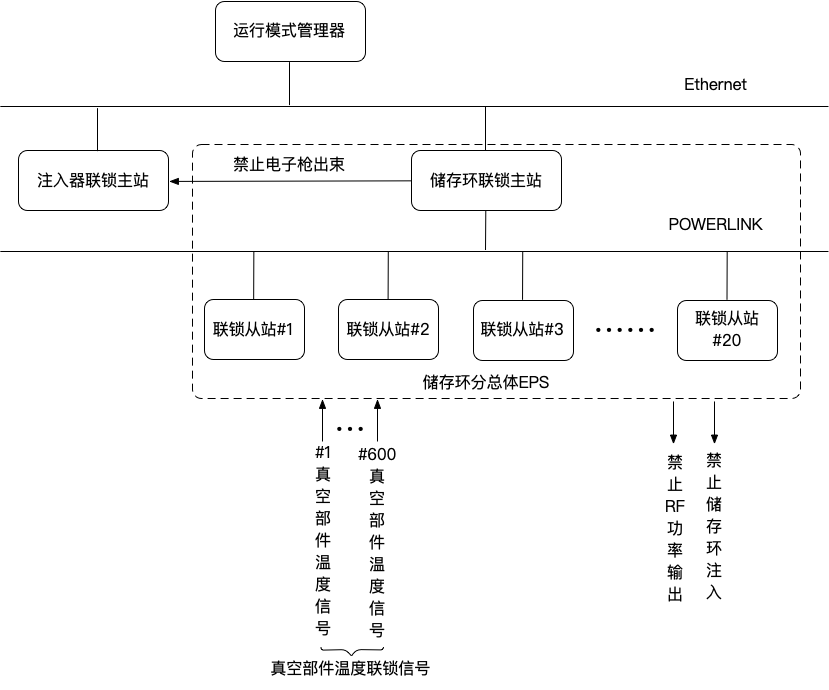
\includegraphics[width=0.975\textwidth]{ring-temp-eps.png}
	\caption{真空部件温度联锁系统结构图}
	\label{fig:ring-temp-eps}
\end{figure}

真空部件温度联锁系统的输入信号是储存环范围内真空盒、光子吸收器和波纹管等真空部件的外壁温度信号,每个联锁从站包括相应区域的真空部件共30个温度信号,全环共600个真空部件温度联锁信号,

图~\ref{fig:linac-vacuum-eps}所示的是真空部件温度联锁系统结构图。当真空盒、光子吸收器和波纹管等部件的外壁温度超过阈值,相应的联锁从站将故障信息提供给联锁主站,经过主站逻辑处理后,通过高频系统从站切断高频功率输出;通过注入系统联锁从站实施禁止储存环注入的保护动作;同时将联锁故障信号传输给注入器联锁主站,通过电子枪从站关闭激光光闸并切断电子枪、调制器和固态放大器时序触发信号。

\subsection{高频联锁系统}

高频联锁系统的任务是对高频系统内的联锁输入信号提供本地保护措施,同时接收来自主站的保护命令为其他系统的联锁故障信号实施保护措施。图~\ref{fig:ring-eps-rf}所示的是高频联锁系统结构图。高频联锁系统由高频从站负责,从站的输入信号包括高频腔冷却水温度/流量信号、高频腔真空度预警/报警信号、高频腔温度信号和高频腔的输入和反射功率,输出保护动作是切断高频功率的输出。

\begin{figure}[!htb]
	\centering
	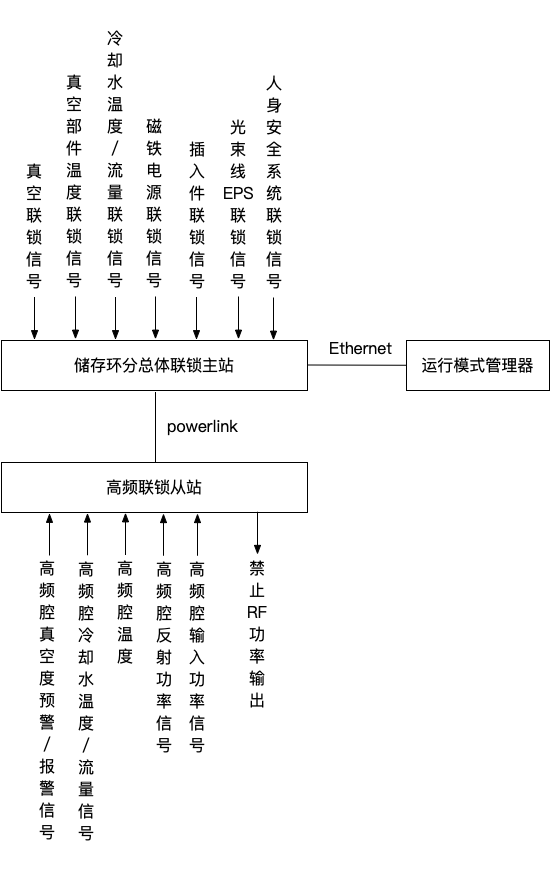
\includegraphics[width=0.7\textwidth]{ring-eps-rf.png}
	\caption{高频联锁系统结构图}
	\label{fig:ring-eps-rf}
\end{figure}

当高频系统内的联锁信号出现故障时,高频腔联锁从站直接实施切断高频功率输出的本地保护动作;同时将联锁故障信号传输给注入器联锁主站,经过联锁主站逻辑处理后通过注入系统联锁从站禁止储存环注入,将联锁故障信号传输给注入器联锁主站,通过电子枪从站实施关闭激光光闸和切断电子枪、调制器和固态放大器序触发信号的保护动作。

当其他系统联锁信号出现故障时,联锁主站需要通过高频系统联锁从站实施相应保护,具体的联锁保护逻辑如下:当储存环分总体内真空度信号、真空部件温度信号、冷却水温度/流量信号、磁铁电源状态信号、来自注入器分总体联锁信号、人身安全系统联锁信号出现故障时,经过主站联锁逻辑处理后,通过高频系统从站实施切断高频功率输出的保护动作。


\subsection{注入联锁系统}

注入联锁系统是对注入系统内的联锁输入信号提供本地保护措施,同时接收来自主站的保护命令为其他系统的联锁故障信号实施保护措施。图~\ref{fig:ring-eps-injection}所示的是注入联锁系统结构图。注入联锁系统由注入从站负责,从站的输入信号包括冲击磁铁和切割磁铁的磁铁电源综合状态信号,输出保护动作是禁止储存环注入。

\begin{figure}[!htb]
	\centering
	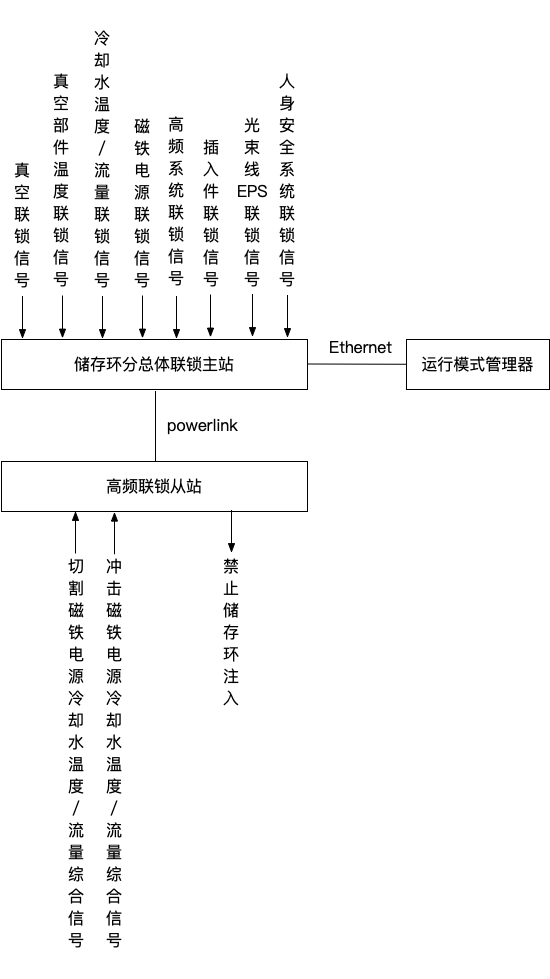
\includegraphics[width=0.65\textwidth]{ring-eps-injection.png}
	\caption{注入联锁系统功能图}
	\label{fig:ring-eps-injection}
\end{figure}

当注入系统内的磁铁电源综合状态信号出现故障时,注入联锁从站直接实施禁止储存环注入的本地保护动作;同时将联锁故障信号传输给储存环联锁主站,经过主站逻辑处理后,通过高频系统联锁从站切断高频功率输出;同时将联锁故障信号传输给注入器联锁主站,通过电子枪从站实施关闭激光光闸和切断电子枪触发信号的保护动作。

当其他系统联锁信号出现故障时,联锁主站需要通过注入系统联锁从站实施相应保护,具体的联锁保护逻辑如下:当储存环分总体内真空度信号、真空部件温度信号、冷却水温度/流量信号、磁铁电源状态信号、来自注入器分总体联锁信号、人身安全系统联锁信号出现故障时,经过主站联锁逻辑处理后,通过高频系统实施禁止储存环注入的保护动作。

\subsection{储存环分总体EPS联锁信号总结}

根据最新的HALF设计参数,我们对储存环分总体EPS的联锁信号进行了初步统计,各系统联锁信号数量如表~\ref{table:4.3}所示。

\begin{table}[!hbt]
  \centering
  \caption{储存环分总体EPS的联锁信号数量统计表}
  \label{table:4.3} 
  \begin{center}
  \begin{tabular}{cccccc}
    \toprule

     系统名称&联锁输入信号&联锁保护信号\\
    \midrule
    真空联锁系统& 120 & 30 \\

    冷却水联锁系统  &500& 0\\
    
    真空部件温度联锁系统  & 600 & 0 \\
    
    磁铁电源联锁系统 &620 & 0\\
    
    高频联锁系统 &2 &1 \\
    
    注入联锁系统  &2& 1\\

    插入件联锁系统 & 20& 0\\

    光束线联锁系统 & 10& 0\\
    
    人身安全系统& 1& 0\\

    总计&1875& 32\\

    \bottomrule
  \end{tabular}
\end{center}
\end{table}

\subsection{储存环设备保护系统实时性能评估}

根据储存环分总体设备保护系统的设计方案,我们同样可以将第~\ref{section:全站FPGA方案的系统设计与开发}节中基于POWERLINK的分布式IO系统作为储存环分总体EPS的原型系统,结合储存环设备保护系统的设计规模和具体联锁信号数量,采用理论计算和网络模拟两种方法对储存环设备保护系统的实时性能进行评估。

\subsubsection{理论计算}

我们首先对储存环分总体的设备保护系统的通信周期进行分析计算。通信周期由等时同步阶段和空闲阶段组成,等时同步阶段的时长可按照公式为~\ref{equation35},其中$T_{sync}$为SoC数据帧同步各从站的时间,根据第~\ref{section:全站FPGA方案通信周期的理论计算}节中对同步阶段的理论分析,$T_{sync}$的最大值一般不超过1$\mu$s。

\begin{equation}
\label{equation35}
T_{ip}=T_{sync}+T_{poll}
\end{equation}

轮询阶段时长$T_{poll}$按照公式~\ref{equation36}来计算,其中$sum_{i=1}^{20}(T_{F(PRes)}^{i}$+$T_{F(PReq)}^{i})$为20个联锁从站的PReq/PRes数据帧的传输时间之和。储存环设备保护系统系统中所有PReq/PRes帧的总数据量($DataSize_{total}^{PReq/PRes}$)可通过公式~\ref{equation37}进行计算,总数据量由PReq/PRes数据帧的帧头帧尾总数据量($DataSize_{total}^{format}$)和PReq/PRes数据帧的应用层总数据量($DataSize_{total}^{user\_data}$)组成。根据第~\ref{subsection:POWERLINK协议的网络模型}节中对POWERLINK数据帧结构的分析,PReq数据帧和PRes数据帧的帧头帧尾大小($DataSize_{format}^{PReq}$,$DataSize_{format}^{PReq}$)均为31Byte,根据公式~\ref{equation38},可得20个联锁从站的PReq/PRes数据帧的帧头帧尾总数据量($DataSize_{total}^{format}$)等于1240Byte。

PReq和PRes数据帧中的应用层数据分别对应于该从站的输出信号和输入信号,考虑到与联锁信号相关的锁存、旁路等预处理状态信号,我们按照一个输入/输出信号的相关数据大小为1Byte来进行计算,根据公式~\ref{equation39},PReq和PRes数据帧中的应用层总数据量即等于系统联锁信号的总数量。
根据表~\ref{table:4.2}的统计结果,储存环设备保护系统中联锁信号的总数量为1907,考虑到保护设备的回读状态信号,这里我们将联锁信号数量翻倍,即按照3814个总联锁信号数量来进行计算。


我们将$DataSize_{total}^{format}$和$DataSize_{total}^{user\_data}$的数值代入公式~\ref{equation37},得到系统中所有PReq/PRes数据帧的总大小为4654Byte,按照千兆以太网的速率进行数据传输,可计算出PReq/PRes数据帧传输时间之和($\sum_{i=1}^{20}(T_{F(PReq)}^{i}+T_{F(PRes)}^{i})$)为50.540$\mu$s。

\begin{equation}
\begin{split}
\label{equation36}
T_{poll}=\sum_{i=1}^{20}(T_{F(PReq)}^{i}+T_{F(PRes)}^{i})+T_{net}^{line}\\
\end{split}
\end{equation}


\begin{equation}
\label{equation37}
DataSize_{total}^{PReq/PRes} = DataSize_{total}^{format}+DataSize_{total}^{user\_data}\\
\end{equation}

\begin{equation}
\begin{split}
\label{equation38}
DataSize_{total}^{format} = 20(DataSize_{format}^{PReq}+DataSize_{format}^{PRes})\\
\end{split}
\end{equation}

\begin{equation}
\begin{split}
\label{equation39}
DataSize_{total}^{user\_data} = sum_{i=1}^{13}(DataSize_{InputSignal}^{i}+DataSize_{outputSignal}^{i})\\
\end{split}
\end{equation}

公式~\ref{equation36}中的$T_{net}^{line}$为储存环设备保护系统的网络组件延时,各联锁从站按照线型拓扑结构相连,$T_{net}^{line}$可按照公式~\ref{equation40}进行计算,其中$T_{c}$为相邻两节点之间网线的传输延时,储存环周长为480m,这里假定各联锁从站按照等距离部署,相邻从站之间的距离为24m,按照5ns/m的传输延时计算,$T_{c}$为0.12$\mu$s。 $T_{hub}$ 、$T_{r-cn}$ 、$T_{r-mn}$参数根据第~\ref{section:全站FPGA方案通信周期的理论计算}节中系统的实测结果,分别为0.661$\mu$s、0.925$\mu$s和1.717$\mu$s,代入公式~\ref{equation40},可得$T_{net}^{line}$为344.946$\mu$s。

\begin{equation}
\begin{split}
\label{equation40}
T_{net}^{line}&=\sum_{i=1}^{20}[2iT_{c}+(2i-1)T_{hub}+T_{r-cn}]+nT_{r-mn}\\
\end{split}
\end{equation}

将$T_{net}^{line}$和$\sum_{i=1}^{20}(T_{F(PReq)}^{i}+T_{F(PRes)}^{i})$的值代入公式~\ref{equation36},可得轮询阶段时长$T_{poll}$为395.486$\mu$s,加上同步阶段的时长$T_{sync}$,则等时同步阶段的时长$T_{ip}$为396.486$\mu$s。

考虑到空闲阶段时长为定值,为传输最大异步数据预留的时间,根据第~\ref{section:全站FPGA方案通信周期的理论计算}节中系统的实测结果为12.920$\mu$s,可得储存环设备保护系统通信周期为409.406$\mu$s。


根据第~\ref{subsection:系统性能测试与分析}节中对测试系统响应时间的分析,耗时最长的响应过程为联锁输入信号从1号从站输入,经过主站处理后,通过20号从站输出保护动作,此过程跨越3个周期,考虑到输入信号的通信等待时间和从站数字隔离器5$\mu$s的信号处理时间,储存环设备保护系统的最长响应时间约为1.643ms。

\subsubsection{网络模拟}

基于OMNeT++仿真平台,我们对储存环设备保护系统进行了建模,模型如图~\ref{fig:20node-model-omnet}所示。

\begin{figure}[!htb]
  \centering
  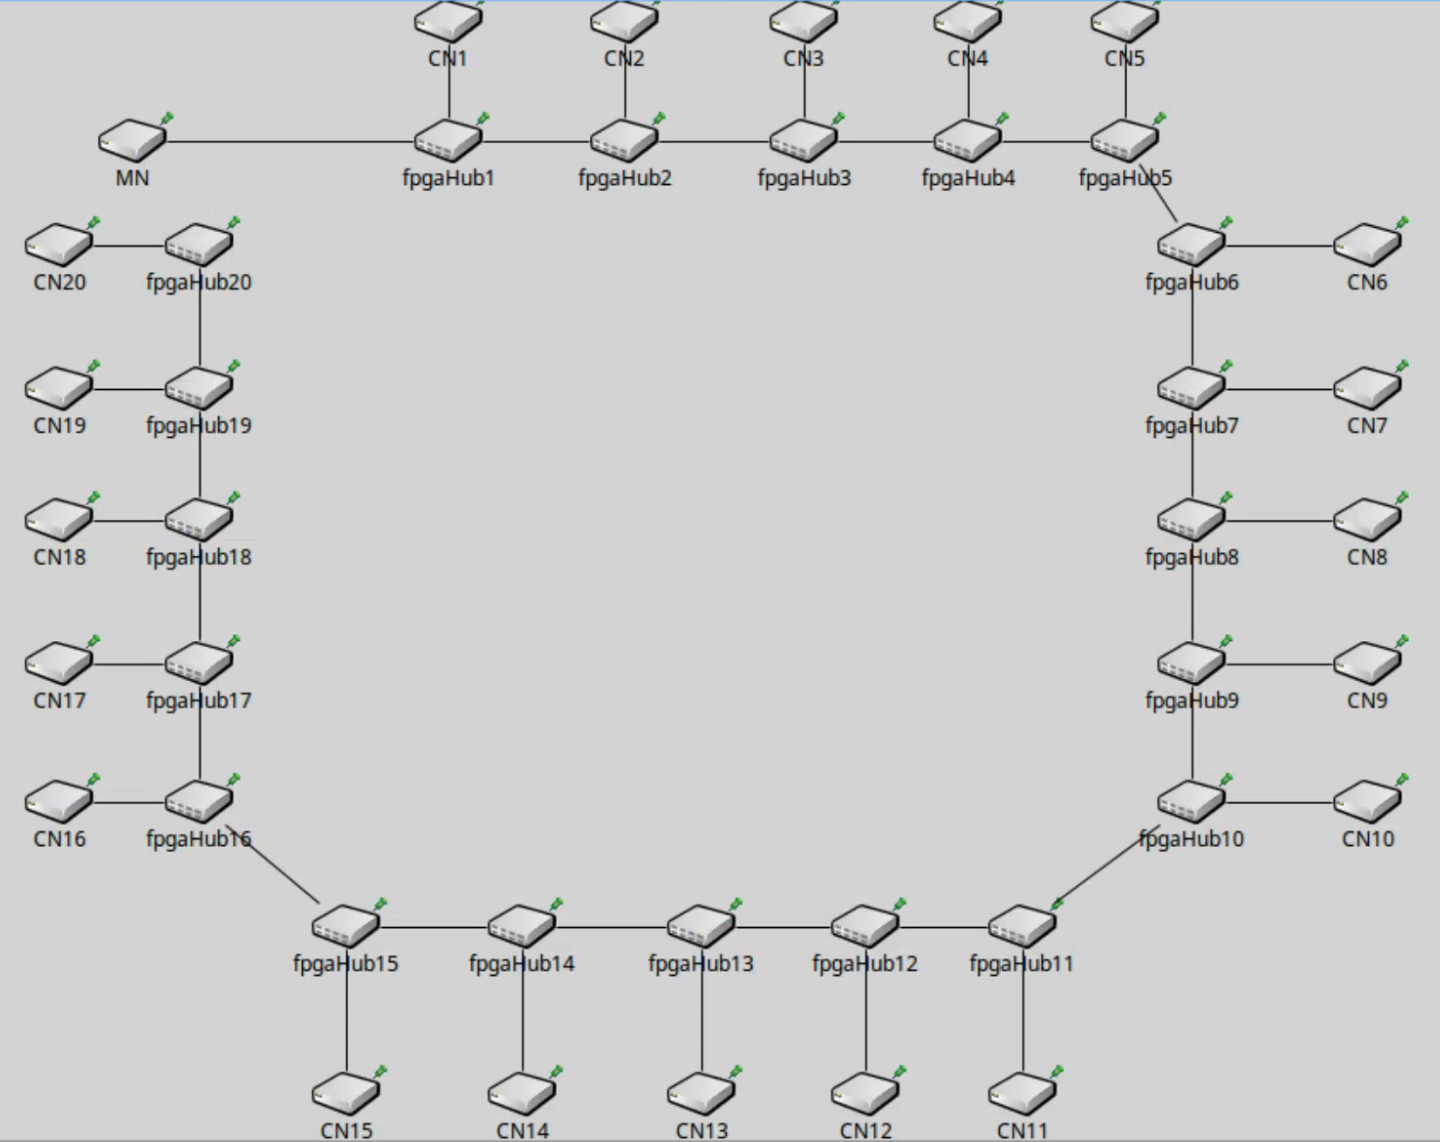
\includegraphics[width=0.85\textwidth]{20node-model-omnet.png}
  \caption{储存环设备保护系统模型}
  \label{fig:20node-model-omnet}
\end{figure}

根据第~\ref{section:全站FPGA方案通信周期的理论计算}中对通信周期的理论分析,各联锁从站被分配的通信时隙($T_{cn-slot}^{i}$)可通过公式~\ref{equation42}和公式~\ref{equation43}计算得到,其中各从站的PReq数据帧和PRes数据帧的传输时间$T_{F(PReq)}$和$T_{F(PRes)}$跟该从站的输入和输出信号数量有关,各从站较为均匀的部署在储存环范围内,这里我们将储存环联锁信号总数量按照各从站进行均分计算,根据表~\ref{table:4.2}的统计结果,储存环设备保护系统中联锁信号的总数量为1907,考虑到输出信号的回读状态信号、运行模式切换信号等相关信号,这里同样将联锁信号数量翻倍,即按照3814个总联锁信号数量来进行计算,则每个从站的联锁信号数量为191。根据公式~\ref{equation44},PReq/PRes帧的帧头帧尾($DataSize_{PReq/PRes}^{i}$)均为21Byte,可得每个从站的PReq/PRes帧的数据量($DataSize_{PReq/PRes}^{i}$)为233Byte。$T_{hub}$ 、$T_{r-cn}$ 、$T_{r-mn}$参数按照第~\ref{section:全站FPGA方案通信周期的理论计算}节中系统的实测结果,分别为0.661$\mu$、0.925$\mu$s和1.717$\mu$s,可以计算出各联锁从站被配置的通信时隙(PResTimeout)。各从站具体配置如下所示:

\begin{equation}
\label{equation41}
DataSize_{PReq/PRes}^{i} = DataSize_{format}^{i}+DataSize_{user\_data}^{i}\\
\end{equation}

\begin{equation}
\label{equation42}
T_{rtd}^{i}=2iT_{c}+(2i-1)T_{hub}+T_{r-cn}
\end{equation}

\begin{equation}
\label{equation43}
T_{cn-slot}^{i}=T_{F(PReq)}^{i}+T_{F(PRes)}^{i}+T_{rtd}^{i}+T_{r-mn}
\end{equation}


\begin{equation}
\label{equation44}
DataSize_{PReq/PRes}^{i} = DataSize_{format}^{i}+DataSize_{user\_data}^{i}\\
\end{equation}

各从站具体配置如下所示,其中PResTimeout为各联锁从站的通信时隙,PReqActPayload为各从站的输出信号大小。

\begin{lstlisting}
<Nodes>
  <Node NodeId="1" PResTimeout="5677ns" PReqActPayload="5byte" />
  <Node NodeId="2" PResTimeout="7237ns" PReqActPayload="6byte" />
  <Node NodeId="3" PResTimeout="8797ns" PReqActPayload="6byte" />
  <Node NodeId="4" PResTimeout="10357ns" PReqActPayload="6byte" />
  <Node NodeId="5" PResTimeout="11917ns" PReqActPayload="6byte" />
  <Node NodeId="6" PResTimeout="13477ns" PReqActPayload="6byte" />
  <Node NodeId="7" PResTimeout="15037ns" PReqActPayload="6byte" />
  <Node NodeId="8" PResTimeout="16597ns" PReqActPayload="6byte" />
  <Node NodeId="9" PResTimeout="18157ns" PReqActPayload="6byte" />
  <Node NodeId="10" PResTimeout="19717ns" PReqActPayload="6byte" />
  <Node NodeId="11" PResTimeout="21277ns" PReqActPayload="6byte" />
  <Node NodeId="12" PResTimeout="22837ns" PReqActPayload="1byte" />
  <Node NodeId="13" PResTimeout="24397ns" PReqActPayload="1byte" />
  <Node NodeId="14" PResTimeout="25957ns" PReqActPayload="6byte" />
  <Node NodeId="15" PResTimeout="27517ns" PReqActPayload="6byte" />
  <Node NodeId="16" PResTimeout="29077ns" PReqActPayload="6byte" />
  <Node NodeId="17" PResTimeout="30637ns" PReqActPayload="6byte" />
  <Node NodeId="18" PResTimeout="32197ns" PReqActPayload="6byte" />
  <Node NodeId="19" PResTimeout="33757ns" PReqActPayload="6byte" />
  <Node NodeId="20" PResTimeout="35317ns" PReqActPayload="1byte" />
</Nodes>
\end{lstlisting}

\begin{figure}[!htb]
  \centering
  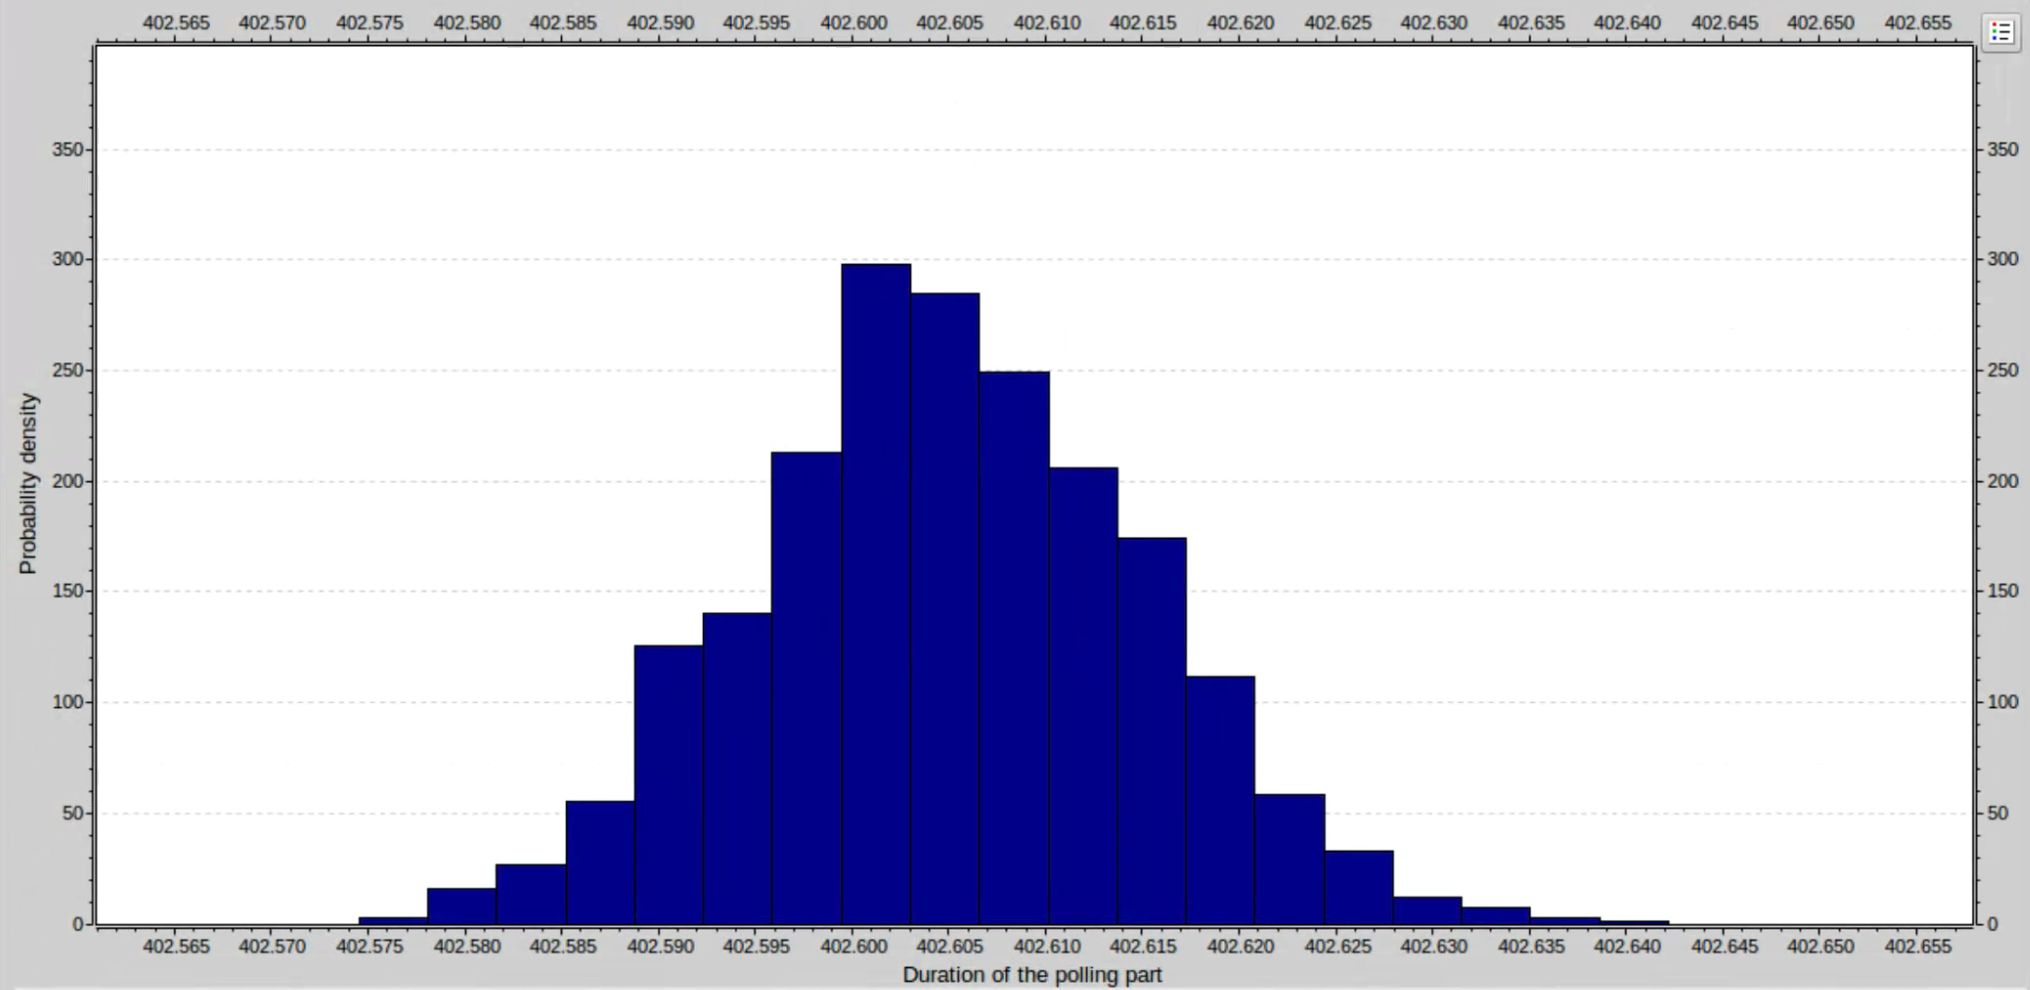
\includegraphics[width=\textwidth]{iso-time-density-20cn-model.png}
  \caption{储存环设备保护系统模型轮询阶段时长的概率密度分布}
  \label{fig:iso-time-density-20cn-model}
\end{figure}

模拟过程持续了大约1000个POWERLINK通信周期。等时同步阶段的概率密度分布绘制在图~\ref{fig:iso-time-density-20cn-model}中,该图表明储存环设备保护系统轮询平均时长为393.379$\mu$s。考虑到同步阶段时长$T_{sync}$最大为1$\mu$s和12.920$\mu$s的空闲时长,可得储存环设备保护系统通信周期为407.279$\mu$s。考虑到输入信号的通信等待时间和从站数字隔离器5$\mu$s的信号处理时间,储存环设备保护系统的最长响应时间约为1.634ms。

 \subsubsection{小结}

我们通过理论计算和仿真模拟的方法两种方法对储存环设备保护系统的实时性能进行了估算,两种方法的计算结果比较相近,通信周期的估算结果分别为409.406$\mu$s和407.279$\mu$s,最大响应时间的的估算结果分别为1.643ms和1.634ms,通过理论计算和仿真模拟的方法两种方法得到的结果较接近,均完全满足设备保护系统响应时间10ms响应时间的需求。

\section{HALF设备保护系统的信息报警}

系统运行过程中出现异常情况时,及时将报警信息发布出来,让工作人员第一时间进行故障维修或隐患排除,对提高系统的可用性是非常重要的。HALF EPS是在EPICS架构下设计的,如图~\ref{fig:halfeps-arch}所示。EPICS社区先后发布过多款报警软件,如ALH、BEAST和Phoebus/Alarms等\cite{alh,Kasemir-2009,Rosati-2017}。Phoebus/Alarms是最新发布的报警软件,由美国橡树岭国家实验室(Oak Ridge National Laboratory,ORNL)的工作人员开发。国家同步辐射实验室在HALF预研工程中对Phoebus/Alarms报警软件进行了研究,并在其基础上根据实际需求进行了二次开发,增加了报警信息网页查询、微信和短信3种报警信息发布方式\cite{chenxin-2019}。

\begin{figure}[!htb]
	\centering
	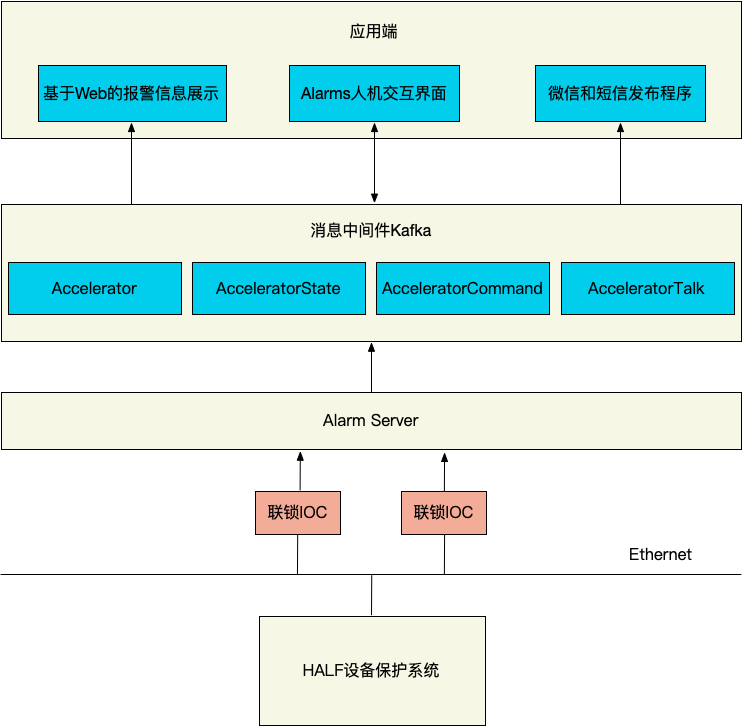
\includegraphics[width=0.6\textwidth]{alarm-eps.png}
	\caption{报警系统架构图}
	\label{fig:alarm-eps}
\end{figure}

图~\ref{fig:alarm-eps}是HALF EPS报警系统的架构图,分为服务端、Kafka、上层应用端等3层。服务端是Alarms的组件Alarm Server。Alarm Server从Kafka中读取报警系统配置文件,然后通过CA协议从联锁IOC中获得相关联锁信号的报警信息,并将相报警信息发送Kafka分布式消息中间件。上层应用端主要由3类模块组成,分别是Phoebus/Alarms中的客户端组件、报警信息查询网页、微信和短信发布程序。

报警信息根据其严重程度进行分为3个等级:严重故障、一般故障和正常状态。严重故障会通过短信和微信及时发送给相关工作人员,在控制界面上以红色标记,可以启动自动保护程序或由工作人员决定处理措施;一般故障不发送短信和微信,仅在控制界面上以黄色标记,给予提醒;正常状态的信息用于描述设备的运行状态,不使用标记颜色。

\section{HALF设备保护系统的历史数据存档与查询}

HALF设备保护系统在运行的过程中,会产生大量与联锁事件相关的数据,包括设备故障数据以及相关的联锁保护数据等,这些存档数据可用于HALF装置故障诊断,对装置的运行维护具有重要意义。HALF装置计划采用Archiver Appliance作为历史数据存档工具,Archiver Appliance是EPICS社区最新发布的数据存档软件\cite{aa-homepage},已应用在国内外多个加速器装置中,如SLAC、NSLS-II、ESS、HLS-II\cite{SHANKAR-2015,KORHONEN-2015,song-2019}等,HALF设备保护系统的联锁事件相关历史数据也会存入基于Archiver Appliance的HALF数据存档与查询系统中。

Archiver Appliance设计了三个数据存储级别,即根据数据产生时间将历史数据划分为短期存储、中期储存和长期存储,如表所示~\ref{table:4.5}。数据首先存入位于读写速度最快的内存中(短期存储),随着时间的推移,逐步迁移至位于读写速度稍慢的本地硬盘(SSD)中(中期存储),最后数据全部存入读写速度最慢的网络存储 (SAN )中 (长期存储)。一般来说,距离越近的数据检索越频繁,因此这样的设计可有效提工作人员查询联锁事件相关历史数据的效率。

\begin{table}[!htb]
	\centering\small
	\caption{Archiver Appliance存储级别}
	\label{table:4.5}
	\begin{center}
	\begin{tabular}{lll}
	  \toprule
	  存储级别   & 数据产生时间   & 存储介质              \\
	  \midrule
	  短期存储 & 几个小时内  & 内存 \\
	  中期存储 & 几天内     & 本地硬盘(SSD)\\
	  长期存储 & 长期       &  网络存储(SAN) \\
	  \bottomrule
	\end{tabular}
	\end{center}
\end{table}

基于Archive Appliance,我们设计了HALF设备保护系统的历史数据存档系统,架构如图~\ref{fig:AA-eps}所示。系统分为数据存档软件和数据可视化应用两个部分,Archive Appliance 作为历史数据存档工具负责收集来自联锁IOC的数据,Archiver Appliance中数据采集引擎通过EPICS Channel Access与联锁IOC中的每个PV建立连接,监测PV值的变化,并将其写入短期存储中。Archiver Appliance内置的迁移模块完成了不同存储级别之间的数据自动迁移,数据检索模块提供了用于数据查询的HTTP/JSON接口。数据可视化应用采用基于web的网页图形界面为操作人员提供历史数据查询功能。

\begin{figure}[!htb]
	\centering
	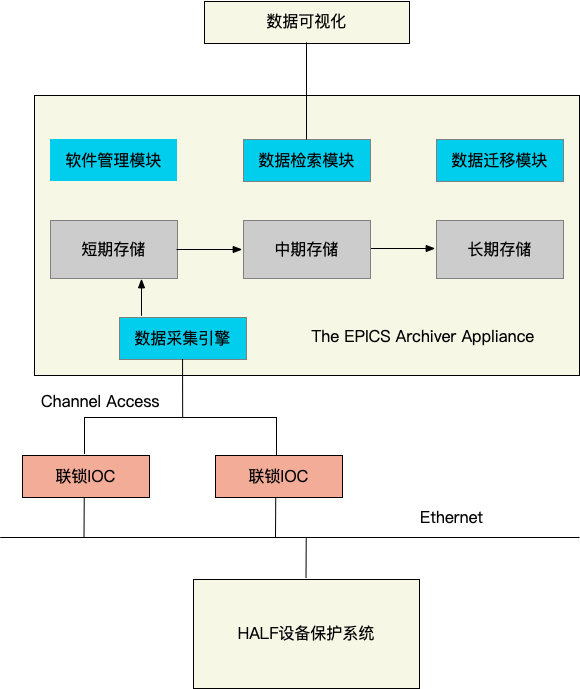
\includegraphics[width=0.5\textwidth]{AA-eps.png}
	\caption{历史数据存档与查询系统图}
	\label{fig:AA-eps}
\end{figure}



